\documentclass[11pt,letterpaper]{article}

% ── Packages ──────────────────────────────────────────────
\usepackage[margin=1in]{geometry}
\usepackage{amsmath,amssymb,amsthm}
\usepackage{mathtools}
\usepackage{booktabs}
\usepackage{enumitem}
\usepackage{hyperref}
\usepackage[dvipsnames]{xcolor}
\usepackage{titlesec}
\usepackage{microtype}
\usepackage{parskip}
\usepackage{tikz}
\usepackage{multicol}
\usetikzlibrary{arrows.meta,positioning,calc,fit,backgrounds}

% ── Formatting ────────────────────────────────────────────
\hypersetup{colorlinks=true, linkcolor=NavyBlue, citecolor=NavyBlue, urlcolor=NavyBlue,
  pdfstartview=FitH}
\titleformat{\section}{\large\bfseries}{\thesection}{1em}{}
\titleformat{\subsection}{\normalsize\bfseries}{\thesubsection}{1em}{}
\titleformat{\subsubsection}{\normalsize\itshape}{\thesubsubsection}{1em}{}

% ── Custom environments ──────────────────────────────────
\newcommand{\caveat}[1]{\par\smallskip\noindent\textcolor{gray}{\textit{Caveat:} #1}\smallskip}
\newcommand{\assumption}[1]{\par\smallskip\noindent\textcolor{BrickRed}{\textit{Assumption:} #1}\smallskip}
\newcommand{\pp}{\,\text{pp}}

% ── Math shortcuts ────────────────────────────────────────
\newcommand{\bfp}{\mathbf{p}}
\newcommand{\bfz}{\mathbf{z}}
\newcommand{\bfy}{\mathbf{y}}
\newcommand{\bfd}{\mathbf{d}}
\newcommand{\bfb}{\mathbf{b}}
\newcommand{\cS}{\mathcal{S}}
\newcommand{\cM}{\mathcal{M}}
\newcommand{\R}{\mathbb{R}}

\begin{document}

% ── Title ─────────────────────────────────────────────────
\begin{center}
{\LARGE\bfseries Neural Field Perceiver}\\[6pt]
{\large Cross-Patient Speech Decoding from Intra-Operative $\mu$ECoG\\via Reprojection-Supervised Spatial Alignment}\\[12pt]
{\normalsize Ben Tang \quad\textbar\quad Greg Cogan Lab, Duke University}\\[4pt]
{\normalsize April 2026 \quad\textbar\quad Version 5}
\end{center}

\medskip\noindent\rule{\textwidth}{0.4pt}\medskip

\noindent This document is a \textbf{technical design document} for the Neural Field Perceiver project.
It unifies the theoretical problem framing, cross-disciplinary foundations from 3D computer vision,
the full architecture specification, uncertainty estimation, and the experimental plan.
Where possible, claims are labeled as \textbf{externally established}
(published literature with citation), \textbf{internally observed} (our experiments, with protocol
noted), or \textbf{working hypotheses} (plausible but unverified). Not every claim carries a label;
the categorization is strongest in Sections~\ref{sec:shared}--\ref{sec:experiments} and should be
treated as a useful habit, not a guarantee of completeness.
Structural assumptions that could be wrong are marked in \textcolor{BrickRed}{red}.

\tableofcontents
\newpage


%% ====================================================================
%%  PART I: PROBLEM FRAMING
%% ====================================================================

\part{Problem Framing}

\section{The Physical Problem}

Each patient's micro-electrocorticography ($\mu$ECoG) array is a \textbf{sparse spatial sample} of neural activity over the cortical surface during speech production. The array is placed subdurally over left ventral sensorimotor cortex (vSMC) during surgery, and its position in standardized brain space (MNI-152) is determined post-hoc via electrode reconstruction (BioImage Suite for DBS patients, Brainlab for tumor patients).

\subsection{The cortical surface, not free 3D space}

The cortex is a folded two-dimensional sheet, not a volume. Let $\cS$ denote the cortical surface embedded in $\R^3$. The high-gamma analytic amplitude (HGA, 70--150\,Hz envelope) is a function on this surface:
\begin{equation}
a: \cS \times \R \to \R
\end{equation}

For patient $i$ with $N_i$ electrodes at cortical surface positions $\{\bfp_j^{(i)}\}_{j=1}^{N_i} \subset \cS$, we observe:
\begin{equation}\label{eq:observation}
\boxed{d_j^{(i)}(t) = a\bigl(\bfp_j^{(i)},\; t\bigr) + \epsilon_j^{(i)}(t)}
\end{equation}
where $\epsilon$ captures measurement noise, electrode impedance variation, and sub-electrode-scale neural activity not resolved by the ${\sim}2$\,mm contact spacing.

In practice, we approximate cortical surface positions with 3D MNI coordinates,
$\bfp_j^{(i)} \approx (x, y, z)_{\text{MNI}}^{(i,j)}$,
which has two consequences:

\begin{enumerate}[leftmargin=2em]
\item \textbf{Euclidean distance in MNI space does not equal geodesic distance on the cortical surface.} Two electrodes 3\,mm apart in MNI may sit on opposite banks of a sulcus, making them functionally distant. For $\mu$ECoG arrays on exposed cortex, the local patch under the array is approximately planar, so within-array Euclidean distances are reasonable. Cross-patient comparisons at larger scales are more affected by folding geometry.

\item \textbf{Surface-based coordinates} (e.g., projection to \texttt{fsaverage}) would better respect cortical geometry than volumetric MNI coordinates. Whether surface reconstructions exist for our patients depends on the BioImage Suite\,/\,Brainlab outputs available.
\end{enumerate}

\textbf{The decoding problem.} Given observations $\{d_j^{(i)}(t)\}$ at approximately known surface positions, infer the phoneme sequence $\bfy = (y_1, y_2, y_3)$ that produced the spatiotemporal pattern.
This is three separate 9-way classifications, one per phoneme position in the non-word token (e.g., /a/, /b/, /e/ for the token /abe/).

\textbf{The cross-patient problem.} Train on patients $\{1, \ldots, K\}$ and decode for a held-out patient $K{+}1$ whose electrodes sample the cortical surface at \emph{different positions}. The observations are not aligned: electrode $j$ on patient $i$ and electrode $j$ on patient $i'$ correspond to different cortical locations. This problem admits several evaluation regimes of increasing difficulty (Section~\ref{sec:eval-regimes}).

\subsection{What makes this hard}

\begin{table}[ht!]
\centering\small
\begin{tabular}{@{}lll@{}}
\toprule
\textbf{Factor} & \textbf{Quantity} & \textbf{Implication} \\
\midrule
Electrodes per patient & 63--201 & Sparse sampling of the cortical field \\
Electrode spacing & ${\sim}2$\,mm & Samples at approximately columnar scale \\
Array offset across patients & 15--25\,mm in MNI & Different cortical regions sampled \\
Array rotation & Variable & Channel indices meaningless across patients \\
Correspondence uncertainty & Several mm & Coordinate-based alignment is approximate \\
Cortical folding variability & Patient-specific & Sulcal geometry differs across individuals \\
Tumor mass effect (subset) & Variable & Macroscopic warping in 6 of 12 patients \\
Trials per patient & 46--178 & Small-data regime for supervised learning \\
Total utterance per patient & ${\sim}1$\,min & Insufficient for single-patient SSL \\
Phoneme vocabulary & 9 classes $\times$ 3 positions & Three 9-way per-position classifications \\
\bottomrule
\end{tabular}
\end{table}


\section{The Shared Dynamics Hypothesis}\label{sec:shared}

Cross-patient decoding is only possible if the cortical field $a(\bfp, t)$ shares structure across patients. We decompose:
\begin{equation}\label{eq:decomposition}
\boxed{a^{(i)}(\bfp, t) = f\bigl(T_i(\bfp),\; t;\; \bfy\bigr) + r^{(i)}(\bfp, t)}
\end{equation}
where:
\begin{itemize}[leftmargin=2em]
\item $f(\cdot, t; \bfy)$ is the \textbf{shared neural field}---the spatiotemporal pattern that phoneme sequence $\bfy$ produces in canonical cortical space.
\item $T_i: \cS_i \to \cS_{\text{canonical}}$ is a \textbf{patient-specific spatial transform} mapping each patient's cortical surface to a canonical reference. MNI normalization is our estimate of $T_i$, but it is imperfect.
\item $r^{(i)}(\bfp, t)$ is a \textbf{patient-specific residual} capturing individual neural organization, signal characteristics, and functional plasticity.
\end{itemize}
The viability of cross-patient decoding depends on the ratio $\|f\| / \|r^{(i)}\|$ at the spatial resolution accessible to our measurements and alignment procedure.

\textbf{How the equations relate to the model.} Equations~\eqref{eq:observation}--\eqref{eq:decomposition} are the physical setup. Section~\ref{sec:manifold} introduces a further idealization (shared observation function on a manifold). The \textbf{implemented model} (Section~\ref{sec:implemented}) relaxes both idealizations: it conditions explicitly on patient identity and does not enforce a strictly shared observation function. The earlier equations motivate the architecture; they are not claims that the model instantiates them exactly.

\subsection{Evidence for shared dynamics}

\subsubsection{Externally established (published literature)}

\textbf{Per-patient input layers + shared temporal backbone is a successful transfer architecture in related settings.} Singh et al.~\cite{singh2025} demonstrate group training with $N{=}25$ sEEG patients: per-patient Conv1D + shared BiLSTM ($2{\times}64$), frozen shared backbone + fine-tuned per-patient layers yields PER 0.49 vs.\ 0.57 single-subject ($p{<}0.001$). Willett et al.~\cite{willett2023} use per-day affine input layer ($256{\to}256$) + shared 5-layer GRU (512 hidden) for day-to-day BCI transfer.

\caveat{Singh's data regime is ${\sim}60$\,min/patient (vs.\ our ${\sim}1$\,min); Conv1D hyperparameters are unreported. Willett is $N{=}1$ with ${\sim}40$\,min/day. The architectural pattern transfers; the hyperparameters do not.}

\textbf{Articulatory somatotopy in vSMC is reproducible within individuals.} Metzger et al.~\cite{metzger2023} show somatotopic organization of speech articulators in one patient with chronic ECoG (253 channels): labial, front tongue, back tongue, and vocalic representations are spatially organized ($p{<}0.0001$), preserved even after 18 years of anarthria. Bouchard et al.~\cite{bouchard2013} demonstrated reproducible articulatory maps in vSMC across 3 participants.

\caveat{Metzger: $N{=}1$ chronic implant. Bouchard: $N{=}3$, standard ECoG. Cross-patient spatial consistency is inferred from anatomical uniformity but not directly measured in a large-scale study.}

\textbf{Articulatory features are a robust encoding basis in vSMC.} Wu et al.~\cite{wu2025} reconstruct speaker-invariant articulatory features from HD-ECoG over vSMC (PCC 0.75--0.80, $N{=}3$), including one intra-operative patient (PCC\,=\,0.76). Anumanchipalli et al.~\cite{anumanchipalli2019} reconstructed continuous articulatory trajectories from motor cortex.

\textbf{MNI coordinates may help cross-patient ECoG transfer.} Chen et al.~\cite{chen2025} (SwinTW) use MNI coordinates and ROI embeddings across 43 ECoG + 9 sEEG subjects, reporting mean PCC\,=\,0.765 on unseen participants in cross-validation.

\caveat{Standard ECoG has ${\sim}10$\,mm spacing, comparable to inter-subject correspondence uncertainty. Our $\mu$ECoG spacing (${\sim}2$\,mm) is finer, meaning coordinates may encode global array position but not resolve within-array relationships.}

\textbf{Motor cortex neural manifold structure is preserved across individuals.} Safaie et al.~\cite{safaie2023} show motor cortex population dynamics during reaching are geometrically similar across monkeys. Gallego et al.~\cite{gallego2020} show low-dimensional manifold dynamics are preserved within individuals across time despite neural turnover.

\caveat{Safaie: limb motor cortex, non-human primates. Gallego: within-individual. Extension to cross-individual speech motor cortex is plausible but untested.}

\subsubsection{Internally observed (our experiments)}

\textbf{Cross-patient supervised transfer produces above-chance decoding.} Our LOPO pipeline achieves PER\,=\,0.762 on held-out S14 (frozen-backbone adaptation, grouped-by-token CV): Stage~1 trains the shared backbone on 9 source patients, Stage~2 freezes Conv1d+BiGRU and adapts only the per-patient read-in, LayerNorm, and head (${\sim}2{,}300$ params). This is well above chance (${\sim}0.89$) but still worse than per-patient PER\,=\,0.737 (same CV, same patient). The gap (2.5\,pp) shows that shared structure in $f$ is exploitable but that patient-specific training on 153 trials still wins---consistent with the residual $r^{(i)}$ being non-negligible.

\textbf{Articulatory bottleneck head improves LOPO decoding.} Consistent with $f$ being organized along articulatory feature dimensions.

\textbf{55 experiments on S14 converge to PER 0.750--0.780.} See Section~\ref{sec:wall} for interpretation.

\textbf{SSL features carry partial structure.} JEPA + LP-FT achieves PER\,=\,0.797 (vs.\ 0.854 basic). Supervised features with the same recipe achieve 0.737.

\subsubsection{Working hypotheses (plausible but unverified)}

The ${\sim}0.76$ PER convergence partly reflects spatial alignment limitations (not isolated from data scarcity or S14-specific effects). MNI coordinates may improve decoding (depends on registration accuracy and whether alignment is binding). Cross-task data pooling~\cite{duraivel2025} is a high-value, low-risk path to more data.


\section{The Neural Manifold Connection}\label{sec:manifold}

\subsection{Two views of the same phenomenon}

The cortical field model and the neural manifold hypothesis are dual descriptions. The bridge is the \textbf{latent articulatory state} $\bfz(t) \in \R^k$:
\begin{equation}\label{eq:obs-function}
\boxed{d_j^{(i)}(t) = g\bigl(\bfp_j^{(i)},\; \bfz(t)\bigr) + r^{(i)}\bigl(\bfp_j^{(i)},\; t\bigr) + \epsilon_j^{(i)}(t)}
\end{equation}
where $g: \cS \times \R^k \to \R$ is a \textbf{shared observation function}---the somatotopic map, and $r^{(i)}$ is the patient-specific residual from Eq.~\eqref{eq:decomposition}. The dynamics on the manifold are phoneme-determined:
\begin{equation}\label{eq:dynamics}
\dot{\bfz}(t) = h\bigl(\bfz(t);\; \bfy\bigr)
\end{equation}

This formulation retains the patient-specific residual $r^{(i)}$ but \textbf{idealizes the shared component}: $g$ is assumed to be the same function for all patients, and $\bfz(t)$ is universal. The viability of cross-patient decoding depends on $\|g\| \gg \|r^{(i)}\|$ at the spatial resolution accessible to our measurements. The implemented model (Section~\ref{sec:implemented}) handles $r^{(i)}$ through patient conditioning ($e^{(i)}$, geometric corrections).

\subsection{The factorization is the key insight}

Without factorization, the shared field $f(\bfp, t; \bfy)$ is an arbitrary function of position, time, and phoneme sequence---predicting neural activity at position $\bfp$ during time $t$ of phoneme sequence $\bfy$ requires learning every (position $\times$ time $\times$ phoneme) combination. The factorization decomposes this into two smaller functions composed through a bottleneck:
\begin{equation}
f(\bfp, t; \bfy) = g\bigl(\bfp,\; \bfz(t)\bigr), \qquad \dot{\bfz}(t) = h(\bfz(t); \bfy)
\end{equation}
\begin{itemize}[leftmargin=2em]
\item $\bfz(t) \in \R^k$ ($k \approx 5$--$8$): the \textbf{articulatory state}---tongue position, lip aperture, voicing, etc. This absorbs \textbf{all time and phoneme dependence}. The dynamics $h$ evolves $\bfz$ according to which phonemes are being produced, but $h$ never sees position.
\item $g(\bfp, \bfz)$: the \textbf{somatotopic map}---given a brain position and an articulatory state, what is the neural activity? This absorbs \textbf{all spatial dependence}. Crucially, $g$ never sees time or phonemes directly---only through $\bfz$.
\end{itemize}
Space and time interact \textbf{only through the low-dimensional bottleneck} $\bfz(t)$. This is analogous to matrix factorization: instead of storing an $(N \times T)$ observation matrix, learn an $(N \times k)$ spatial basis and a $(k \times T)$ temporal basis. The bottleneck is what makes the problem tractable with 63--201 electrodes.

\subsection{Articulatory manifold dimensionality}

\begin{table}[ht!]
\centering\small
\begin{tabular}{@{}llc@{}}
\toprule
\textbf{Contrast} & \textbf{Phonemes distinguished} & \textbf{Dim.} \\
\midrule
Place of articulation & labial (b,p,v) vs.\ velar (g,k) & ${\sim}2$ \\
Manner & stop vs.\ fricative vs.\ vowel & ${\sim}2$ \\
Voicing & voiced (b,g,v) vs.\ voiceless (k,p) & ${\sim}1$ \\
Vowel height & low (a,\ae) vs.\ high (i,u) & ${\sim}1$ \\
Vowel backness & front (\ae,i) vs.\ back (a,u) & ${\sim}1$ \\
\midrule
\textbf{Effective dimension} & & $\mathbf{{\sim}5\text{--}8}$ \\
\bottomrule
\end{tabular}
\end{table}

\noindent These dimensions are heuristic (the factors are correlated, not orthogonal) and do not by themselves establish identifiability---unknown transforms, noise, and patient residuals remain.
However, the effective dimension is far below electrode count (63--201), suggesting the problem is \textbf{not obviously underdetermined under a low-dimensional latent hypothesis}.

\subsection{Cross-patient transfer as manifold alignment}

Each patient's array gives a different projection of the shared latent state. As a \textbf{toy linear approximation} (not a claim about the true relationship):
\begin{equation}
\bfd^{(i)}(t) \approx W^{(i)} \bfz(t) + \boldsymbol{\epsilon}^{(i)}
\end{equation}
where $W^{(i)} \in \R^{N_i \times k}$ is determined by electrode positions. In practice, $W^{(i)}$ also absorbs patient-specific physiology, gain differences, pathology effects, and preprocessing artifacts.
MNI coordinates provide the geometric relationship between projections a priori, rather than requiring post-hoc alignment methods (CCA, Procrustes, CORAL). Spalding's PCA+CCA baseline achieves 0.31 balanced accuracy~\cite{spalding2025}; our CORAL and CCA auxiliary losses during LOPO training produced PER\,$\approx$\,0.76---no better than the baseline without them.


\section{Decomposing Cross-Patient Variation}

\subsection{The spatial transform \texorpdfstring{$T_i$}{Ti}}

\begin{equation}\label{eq:transform}
T_i(\bfp) = A_i \cdot \bfp + \bfb_i + \delta_i(\bfp)
\end{equation}
\begin{itemize}[leftmargin=2em]
\item $A_i \in \R^{3 \times 3}$: rigid or affine (rotation, scaling). MNI normalization estimates this.
\item $\bfb_i \in \R^3$: translation (15--25\,mm array placement offset).
\item $\delta_i(\bfp)$: nonlinear residual---sulcal geometry, local folding, \textbf{tumor mass effect} (geometric mapping error in 6/12 patients).
\end{itemize}

\subsection{Inter-subject correspondence uncertainty}

Not a fixed constant. Sources: native-space localization (sub-mm), brain shift correction (variable), atlas warping (dominant). Net: several mm for healthy anatomy, more near tumors.
\begin{itemize}[leftmargin=2em]
\item At somatotopy scale (${\sim}15$--$20$\,mm): reliable.
\item At electrode spacing (${\sim}2$\,mm): unreliable.
\item In between (${\sim}5$--$10$\,mm): partially informative.
\end{itemize}

\subsection{The patient-specific residual \texorpdfstring{$r^{(i)}$}{r(i)}}

Captures: (1)~fine-grained neural organization varying across individuals; (2)~signal characteristics (impedance, contact, SNR); (3)~functional plasticity (accent, articulatory habits); (4)~pathology-specific effects (Parkinson's excitability changes, tumor-adjacent reorganization).


\section{What Our Experiments Reveal}\label{sec:experiments}

\subsection{The evaluation recipe dominates at this data scale}

\begin{table}[ht!]
\centering\small
\begin{tabular}{@{}lllr@{}}
\toprule
\textbf{Component} & \textbf{Category} & \textbf{Cumulative PER} & \textbf{$\Delta$} \\
\midrule
Baseline (CE, mean-pool) & -- & 0.872 & -- \\
+ Label smoothing 0.1 & Training & 0.831 & $-4.1\pp$ \\
+ Per-position heads + dropout & Training & 0.819 & $-1.2\pp$ \\
+ Mixup $\alpha{=}0.2$ & Training & 0.802 & $-1.7\pp$ \\
+ Weighted $k$-NN ($k{=}10$) & Evaluation & 0.781 & $-2.1\pp$ \\
+ TTA (16 augmented copies) & Evaluation & 0.767 & $-1.4\pp$ \\
+ Articulatory + CE dual head & Evaluation & 0.737 & $-3.0\pp$ \\
\bottomrule
\end{tabular}
\end{table}

\noindent These improvements are \textbf{cumulative}, not independent ablations---each row adds to the previous. The ordering affects attribution: label smoothing's $-4.1\pp$ may partly reflect gains that would accrue to other components under a different ordering. The full recipe reduces PER from 0.872 to 0.737 ($-13.5\pp$ total). At this data scale, evaluation-time methods extract substantial additional signal from the learned representation.

\caveat{All improvements measured on S14 grouped-by-token 5-fold CV; per-fold effects are large (${\pm}0.05$), so improvements ${<}2\pp$ may not replicate on other patients.}

\subsection{Multi-scale temporal structure is validated}

Multi-scale temporal encoding (stride 3+5+10) was the single best architectural improvement (PER $0.766 \to 0.750$). The three scales correspond to fast transitions (${\sim}15$\,ms), syllable dynamics (${\sim}25$\,ms), and phoneme-level patterns (${\sim}50$\,ms).

\caveat{Validated with the current BiGRU backbone. Optimal stride values may differ for the transformer temporal encoder proposed here; re-validation is needed (Section~\ref{sec:temporal}).}

\subsection{SSL features carry partial structure}

All SSL methods produce near-chance PER (0.85--0.91) under basic evaluation. JEPA + LP-FT achieves 0.797. SSL features are non-trivial but far weaker than supervised features.

\subsection{The \texorpdfstring{${\sim}$0.76}{~0.76} PER convergence on S14}\label{sec:wall}

55 experiments converge to PER 0.750--0.780. \textbf{Attributing this to any single bottleneck would be premature}:
\begin{enumerate}[leftmargin=2em]
\item \textbf{S14 is no longer held-out.} 55+ architectures evaluated $\Rightarrow$ it functions as a validation set.
\item \textbf{Measurement noise.} ${\sim}30$ samples per fold $\Rightarrow$ ${\pm}0.05$ PER noise. Differences ${<}2\pp$ are within noise.
\item \textbf{Target-data scarcity.} S14 has 153 trials. Stage~2 contributes only ${\sim}1.6\pp$.
\item \textbf{Spatial alignment may be one factor.} Not isolated as \emph{the} bottleneck.
\end{enumerate}


\section{The Case for MNI Coordinates}

\subsection{Currently unused information}

The current pipeline uses per-patient Conv2d on grid topology. Each Conv2d is independent. The model has \textbf{zero information} about cross-patient spatial relationships. The shared backbone implicitly assumes feature alignment across patients---anatomically false for independent per-patient encoders.

\subsection{What coordinates may provide}

Knowing $\bfp_j^{(i)}$ allows learning $g$ as a shared function. Concretely: (1)~identifying which articulatory zone each electrode samples; (2)~sharing representations across patients at similar positions; (3)~contextualizing variable coverage.

\subsection{What coordinates do NOT guarantee}

Coordinates help only if correspondence uncertainty is small enough relative to somatotopic scale, the architecture exploits them, and spatial alignment is actually binding. \textbf{Their value must be demonstrated empirically.}


%% ====================================================================
%%  PART II: CROSS-DISCIPLINARY FOUNDATIONS
%% ====================================================================

\part{Cross-Disciplinary Foundations}

\section{The Multi-View Reconstruction Analogy}\label{sec:analogy}

Inspired by holistic performance capture~\cite{wang2025}, the cross-patient decoding problem maps structurally to \textbf{fitting a parametric 3D model to 2D observations from multiple viewpoints}.

\subsection{The pose estimation mapping}

\begin{table}[ht!]\centering\small
\begin{tabular}{@{}p{0.41\textwidth}c p{0.45\textwidth}@{}}
\toprule
\textbf{3D Pose Estimation} & & \textbf{Neural Field Decoding} \\
\midrule
3D body model (SMPL mesh) & $\leftrightarrow$ & Shared neural field $g(\bfp, \bfz)$ on cortex \\[3pt]
Pose parameters $\theta$ & $\leftrightarrow$ & Articulatory state $\bfz(t)$ \\[3pt]
Shape parameters $\beta$ & $\leftrightarrow$ & Patient embedding $e^{(i)}$ \\[3pt]
Camera extrinsics $[R \mid t]$ & $\leftrightarrow$ & MNI offset $\Delta^{(i)}$ (+ optional $\omega^{(i)}$) \\[3pt]
Camera intrinsics $K$ & $\leftrightarrow$ & Per-patient gain/bias \\[3pt]
2D keypoints $x_j$ & $\leftrightarrow$ & Electrode observations $d_j^{(i)}(t)$ \\[3pt]
Projection function $\pi(\cdot)$ & $\leftrightarrow$ & Observation function $g(\cdot)$ \\[3pt]
\textbf{Reprojection loss} $\|\pi(V) - x\|^2$ & $\leftrightarrow$ & \textbf{Reprojection loss} $\|g(\bfp{+}\Delta, \hat{\bfz}) - d\|^2$ \\
\bottomrule
\end{tabular}
\end{table}

\subsection{What the analogy reveals}

\textbf{Why alignment-based methods struggle:} CCA/Procrustes/CORAL align feature-space statistics---works for similar viewpoints, but 15--25\,mm placement offsets mean the underlying features are genuinely different, not just rotated. Per-patient SpatialConv is a separate 3D model per camera---no sharing. Our approach is \textbf{structurally analogous to Structure from Motion}: jointly estimate shared structure and all camera parameters.

\textbf{Why reprojection loss beats arbitrary SSL:} JEPA/VICReg/masked reconstruction used physically meaningless targets. Reprojection is geometrically grounded: ``if your latent estimate is correct, you should predict what every electrode observes.'' Self-supervised but geometrically constrained.

\subsection{Where the analogy breaks}\label{sec:disanalogies}

The mapping is structural, not exact. Three important disanalogies:

\begin{enumerate}[leftmargin=2em]
\item \textbf{Each patient is a different ``scene,'' not a different camera on the same scene.} In multi-view reconstruction, all cameras observe the SAME 3D scene simultaneously. Our patients are observed independently, at different times, producing different spatiotemporal patterns due to $r^{(i)}$. The shared structure $f$ exists but is weaker than multi-view photometric consistency. The reprojection loss is therefore noisier---it must reconstruct through patient-specific residual, not just geometric projection.

\item \textbf{Reprojection is electrode-sparse, not pixel-dense.} A $256{\times}256$ image provides 65K reprojection constraints per view. Our 63--201 electrodes provide 100--1000$\times$ fewer constraints per frame. The reprojection signal per frame is thin; it aggregates value primarily across the temporal dimension ($T {\approx} 200$ frames/trial $\times$ 1315 trials).

\item \textbf{The ``scene'' changes every frame.} In static reconstruction, the scene is fixed across views. Here, $\bfz(t)$ changes continuously, so each frame is a different scene for reprojection. This is closer to \textbf{dynamic scene reconstruction}---but the temporal structure is phoneme-specific and short-lived (${\sim}1$\,s trials), not a persistent evolving scene.
\end{enumerate}

\noindent These disanalogies mean: the reprojection loss will be noisier and less constraining than its vision analog; geometric inductive biases (distance bias, bilinear factorization) must compensate; and the reprojection loss is a useful regularizer but \textbf{should not be expected to carry the architecture} the way photometric loss carries NeRF. The supervised classification loss remains primary.

\textbf{Transfer criterion.} We adopt 3D vision patterns only when the following structural property holds: the component solves a problem of sparse, geometrically-referenced observations of a shared underlying field, which is our problem regardless of the source domain. Where the analogy demands dense observations, persistent scenes, or exact photometric consistency, we either adapt or drop the pattern.

\section{Transferable Patterns from 3D Vision (2024--2026)}

\subsection{The field's trajectory: per-scene \texorpdfstring{$\to$}{to} feed-forward \texorpdfstring{$\to$}{to} foundation model}

Our architecture sits at step 2 (feed-forward). Key transferable patterns:

\textbf{VGGT}~\cite{wang2025}: joint 3D attribute prediction from variable-length views. Structural precedent for Perceiver jointly estimating latent state + alignment.

\textbf{LVSM}~\cite{jin2024}: encoder-decoder with fixed latent tokens vs.\ decoder-only. Decoder-only wins with enough data; explicit structure wins at small scale. \textit{Motivates our structured approach for ${\sim}1300$ trials.}

\textbf{MMGN}~\cite{xiong2024}: continuous field reconstruction from sparse, irregularly sampled sensors using factorized spatiotemporal basis. Our bilinear decoder is structurally related (Section~\ref{sec:obs-decoder}).

\textbf{SPARF}~\cite{truong2023}: NeRF from sparse and noisy poses. Directly analogous: our MNI coordinates are noisy poses; our electrodes are sparse views.

\textbf{Senseiver}~\cite{jha2023}: Perceiver IO for field reconstruction from sparse sensors---structurally related to our spatial encoder.

\subsection{Architectural pattern validation}

\begin{table}[ht!]\centering\small
\begin{tabular}{@{}p{0.38\textwidth}p{0.56\textwidth}@{}}
\toprule
\textbf{Our component} & \textbf{Same pattern in vision} \\
\midrule
Perceiver cross-attention (virtual $\to$ actual) & Canonical-to-observation tokens (LRM, LVSM) \\
Virtual electrodes at learnable positions & Triplane NeRF / fixed latent tokens \\
MNI distance-biased attention & Geometry-aware attention (GraphSplat, MVSplat) \\
Bilinear decoder $\hat{d} = \phi(\bfp)^\top\psi(s)$ & Spatiotemporal factorization (MMGN) \\
Reprojection loss & Photometric loss (NeRF/3DGS family) \\
Learnable per-patient $\Delta$ & Learnable camera extrinsics (SPARF, AnySplat) \\
Patient embedding $e^{(i)}$ & Per-scene latent code (CodeNeRF) \\
Electrode masking & View dropout / masked pretraining (MAE) \\
Structured inductive bias for small data & Explicit geometry at small scale (LVSM) \\
\bottomrule
\end{tabular}
\end{table}

\subsection{What we are correctly NOT doing}

Diffusion priors (need millions of scenes), 4D Gaussian primitives (trials are independent events), foundation model scale (1300 trials may struggle to support ${>}200$K params---our budget is at the edge), decoder-only architecture (needs massive data), contrastive SSL (failed in our experiments).

\subsection{The data scale gap}

\begin{table}[ht!]\centering\small
\begin{tabular}{@{}lll@{}}
\toprule
& \textbf{3D Vision} & \textbf{Our Problem} \\
\midrule
Training scenes/patients & 50K--1M+ & ${\sim}20$ patients \\
Observations per scene & 10--100+ images (M pixels) & 63--201 electrodes \\
Total data & TB scale & ${\sim}240$\,MB \\
Parameter budget & 50M--500M+ & ${\sim}200$K \\
\bottomrule
\end{tabular}
\end{table}

\noindent This gap means: we \textbf{must} use strong geometric inductive biases; the reprojection loss is valuable but electrode-sparse (Section~\ref{sec:disanalogies}); and our ${\sim}200$K architecture is appropriately small. The field's finding that explicit geometric structure helps at small scale motivates this design choice, though the transfer from vision to neural data is unverified.


\section{Lessons from Video Models and Spatiotemporal Autoencoders}\label{sec:video-lessons}

The 3D vision analogy (Section~\ref{sec:analogy}) motivates the spatial architecture, but our data has a critical dimension that static 3D reconstruction lacks: \textbf{temporal dynamics}. Recent video understanding models (2024--2026) address exactly this---learning joint spatiotemporal representations from sequential observations---and three findings are directly relevant.

\subsection{Don't separate spatial and temporal encoding}

Our architecture processes each time frame independently through the spatial encoder, then feeds the sequence to a temporal encoder. This strict separation means spatial encoding gets \textbf{no temporal context}---a known weakness (Section~\ref{sec:implemented}).

State-of-the-art video models reject this separation:
\begin{itemize}[leftmargin=2em]
\item \textbf{Recurrent Video Masked Autoencoders} (RVM)~\cite{rvm2025}: uses a recurrent transformer to aggregate dense image features \emph{over time during spatial encoding}. RVM-L/H outperform VideoMAE v2 and DINOv2 at giant scale by ${>}10\%$, with much better temporal consistency. The key insight: temporal context during spatial encoding produces more stable representations than post-hoc temporal processing.
\item \textbf{MAE-ST}~\cite{maest2025}: a 3D masked autoencoder with spatiotemporal transformer for \textbf{4D fMRI data}---the closest published architecture to our problem. ViT extracts spatial features, temporal transformer extracts temporal features, decoder reconstructs masked fMRI sequences. Achieves SOTA on HCP task fMRI and ADHD-200 classification.
\end{itemize}

\textbf{Implication for us:} Replace the strict spatial$\to$temporal pipeline with \textbf{interleaved spatiotemporal attention}---alternating spatial attention (electrodes attend within a time window) and temporal attention (each electrode attends across windows) within each layer, following the ViViT/TimeSformer factorized pattern. This gives temporal context to spatial encoding at every stage without the full $O((N{\cdot}T)^2)$ cost of joint attention.

\subsection{Masked spatiotemporal tubes, not per-frame electrode masking}

Our current design masks random electrodes within each frame independently. VideoMAE~\cite{videomae2022} introduced \textbf{tube masking}: mask an entire spatiotemporal tube (the same spatial patch tracked across multiple frames). This forces the model to interpolate in both space \textbf{and} time simultaneously.

\textbf{Implication for us:} Mask an electrode across a contiguous time window (e.g., drop electrode $j$ for frames $t$ through $t{+}k$). The reprojection loss then requires the model to reconstruct electrode $j$'s activity from (a)~nearby electrodes at the same time, and (b)~electrode $j$ at adjacent times. This is strictly harder than per-frame masking and produces representations that encode both spatial and temporal structure.

\subsection{Mamba for efficient spatiotemporal processing}

Joint spatiotemporal processing increases the token count (e.g., 150 electrodes $\times$ 30 windows $= 4{,}500$ tokens). The \textbf{Video Mamba Suite}~\cite{videomamba2025} demonstrates that state space models (SSMs) match or beat Transformers across 12 video tasks while maintaining \textbf{linear complexity} in sequence length---exactly where the efficiency advantage matters for our token counts.

\textbf{Implication for us:} If we move to joint spatiotemporal processing, Mamba's $O(N)$ scaling (vs.\ Transformer's $O(N^2)$) makes the increased token count tractable. This is an architectural option, not a requirement---factorized attention is also viable at our scale.

\subsection{Summary: architectural evolution}

\begin{table}[ht!]\centering\small
\begin{tabular}{@{}p{0.28\textwidth}p{0.30\textwidth}p{0.32\textwidth}@{}}
\toprule
& \textbf{Current design} & \textbf{Video-inspired variant} \\
\midrule
Spatial encoding & Per-frame, no temporal context & Interleaved spatial + temporal attention \\
Masking & Per-frame electrode dropout & Spatiotemporal tube masking \\
Temporal backbone & Separate transformer & Integrated in every layer \\
Complexity & $O(L \cdot N)$ per frame & $O(N \cdot T)$ factorized, or $O(N{\cdot}T)$ Mamba \\
\bottomrule
\end{tabular}
\end{table}

\noindent The current design (Section~\ref{sec:implemented}) is the simpler starting point. The video-inspired variant is a natural evolution if single-frame spatial encoding proves insufficient. The rest of the pipeline (bilinear decoder, reprojection loss, phoneme classification) is unchanged---only the encoder architecture swaps.

\caveat{MAE-ST uses fMRI (${\sim}2$\,mm voxels, ${\sim}0.5$\,Hz TR, whole-brain coverage), while we use $\mu$ECoG (${\sim}2$\,mm contacts, 200\,Hz, focal cortical coverage). The spatial resolution is similar but temporal resolution differs by $400\times$ and spatial coverage by ${\sim}100\times$. The architectural patterns transfer; the hyperparameters (masking ratios, window sizes, layer counts) will not.}


\section{Uncertainty Estimation}\label{sec:uncertainty}

\subsection{From binary to continuous weighting}

The current pipeline has a binary mechanism: significant channel selection (keep/drop). A continuous weighting scheme replaces this with per-electrode importance scores.

\subsection{Two types of uncertainty}

\textbf{Aleatoric} (irreducible): ``This electrode position tends to have low SNR.'' Per-electrode, does not decrease with more data.

\textbf{Epistemic} (reducible): ``We lack data in this cortical region.'' Per-position, decreases with more patients.

\subsection{Recommended uncertainty stack}

\subsubsection{Tier 1: Minimal implementation, high value}

\textbf{Beta-NLL loss}~\cite{seitzer2022}. Replace MSE reprojection with learned per-electrode variance:
\begin{equation}
\mathcal{L}_{\text{reproj}}^{\text{UQ}} = \frac{1}{2}\Bigl(\log \hat{\sigma}_j^2 + \frac{(d_j - \hat{d}_j)^2}{\hat{\sigma}_j^2}\Bigr) \cdot \bigl(\hat{\sigma}_j^2\bigr)^{0.5}_{\text{sg}}
\end{equation}
\textbf{Scope}: Beta-NLL affects the \textbf{training loss only}---it downweights reprojection gradients from noisy electrodes, preventing them from distorting the encoder. It does \textbf{not} directly modulate attention weights at inference time.

\textbf{MC Dropout at inference}~\cite{gal2016}. Keep dropout active, 10--20 passes, variance $=$ epistemic uncertainty. Remove dropout from output layer.

\textbf{Conformal prediction}~\cite{angelopoulos2021}. Post-hoc prediction \textbf{sets} with distribution-free coverage guarantees. Within each outer CV fold, after model selection on the inner validation split, a \textbf{dedicated calibration subset} (10\% of the training fold, disjoint from the inner validation used for checkpoint selection) produces nonconformity scores. The calibration set is never used for training or model selection, preserving the exchangeability assumption required for the coverage guarantee. Potential interpretability value: ``model thinks /b/ or /p/ (both labial stops)''---the confusion structure itself is informative.

\subsubsection{Tier 2: Moderate implementation}

\textbf{Evidential regression} (NIG prior): single-pass decomposed aleatoric + epistemic per electrode. \textbf{Probabilistic virtual electrodes} (pixelSplat-style): predict latent distributions, uncertainty propagates through the pipeline.

\subsection{How uncertainty connects to the architecture}\label{sec:uq-flow}

\begin{center}
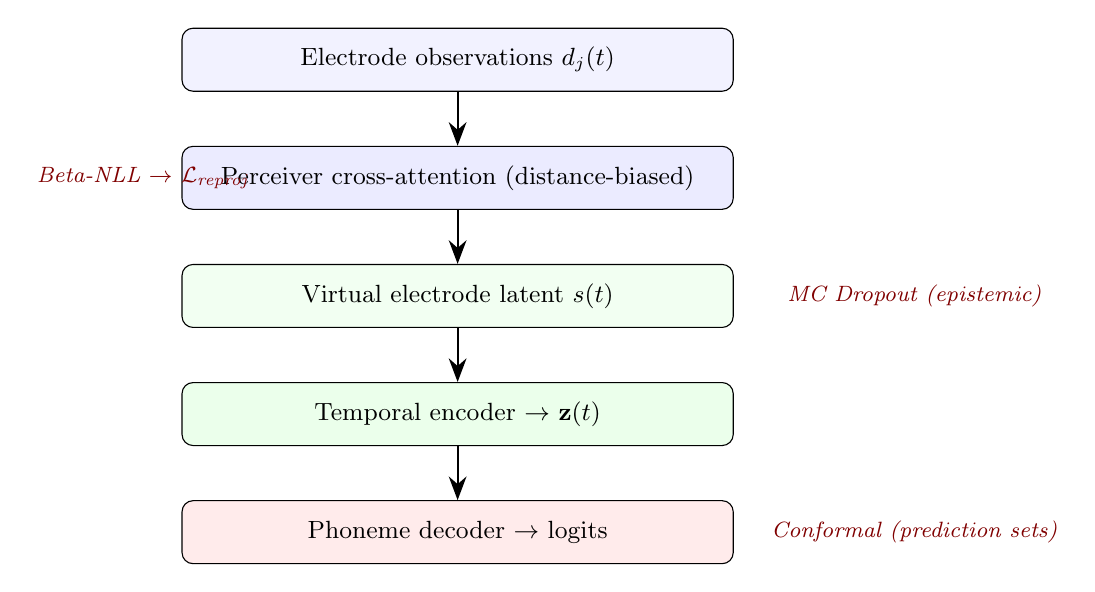
\begin{tikzpicture}[
  box/.style={draw, rounded corners, minimum width=7cm, minimum height=0.8cm, align=center, font=\small},
  uq/.style={font=\footnotesize\itshape, text=Maroon},
  arrow/.style={-{Stealth[length=3mm]}, thick}
]

\node[box, fill=blue!5] (elec) at (0, 0) {Electrode observations $d_j(t)$};

\node[box, fill=blue!8] (perceiver) at (0, -1.5) {Perceiver cross-attention (distance-biased)};

\node[box, fill=green!5] (latent) at (0, -3) {Virtual electrode latent $s(t)$};
\node[uq] (uq2) at (5.8, -3) {MC Dropout (epistemic)};

\node[box, fill=green!8] (temporal) at (0, -4.5) {Temporal encoder $\to$ $\bfz(t)$};

\node[box, fill=red!8] (phoneme) at (0, -6) {Phoneme decoder $\to$ logits};
\node[uq] (uq3) at (5.8, -6) {Conformal (prediction sets)};

\node[uq] (uq4) at (-4, -1.5) {Beta-NLL $\to$ $\mathcal{L}_{\text{reproj}}$};

\draw[arrow] (elec) -- (perceiver);
\draw[arrow] (perceiver) -- (latent);
\draw[arrow] (latent) -- (temporal);
\draw[arrow] (temporal) -- (phoneme);

\end{tikzpicture}
\end{center}

\noindent Beta-NLL affects training gradients (left). MC Dropout captures model uncertainty. Conformal prediction gives calibrated prediction sets. Each mechanism has a distinct scope---they are complementary, not redundant.


%% ====================================================================
%%  PART III: ARCHITECTURE
%% ====================================================================

\part{Architecture Design}

\section{Spatial vs.\ Temporal Dynamics: Design Rationale}\label{sec:spatial-temporal}

The observation model (Eq.~\ref{eq:obs-function}) decomposes into a \textbf{static} spatial component and a \textbf{dynamic} temporal component. This decomposition is physical, not architectural---it follows from the structure of the data. The architecture must decide how to respect or ignore this separation.

\subsection{The spatial problem is static}

The somatotopic map $g(\bfp, \bfz)$---which brain position encodes which articulatory feature---does \textbf{not change during a trial}. Lip motor cortex encodes lip state at $t{=}0$ and at $t{=}500$\,ms. What changes is $\bfz(t)$, the articulatory state being fed through that map. Therefore:

\textbf{Spatial inversion} ($d_j(t) \to \bfz(t)$) is a \textbf{time-invariant function}. Given electrode readings at known positions at any single moment, the task is always the same: invert $g$ to recover the current articulatory state. The spatial encoder should learn this static mapping.

\textbf{Cross-patient alignment is purely spatial.} Different patients have electrodes at different positions sampling the \textbf{same static map} $g$. The alignment challenge---``S14's channel 50 and S22's channel 80 sample the same cortical region''---is geometric and time-invariant. It depends on electrode positions (which do not change during a trial), not on temporal dynamics.

\subsection{The temporal problem is dynamic but shared}

The articulatory trajectory $\bfz(t)$ evolves during speech: tongue moves, lips open/close, voicing starts/stops. This trajectory is \textbf{phoneme-determined} and \textbf{approximately shared across patients}---the same phoneme /b/ produces a similar $\bfz(t)$ trajectory regardless of which patient speaks it (modulo speaking rate and accent).

Temporal similarity provides a \textbf{second source of cross-patient alignment}: even if spatial alignment is imperfect, patients producing the same phoneme should have similar temporal trajectories through the shared latent space. But this alignment comes through the temporal encoder (shared dynamics), not the spatial encoder (shared geometry).

\subsection{The noise argument for temporal context in spatial encoding}

The physics supports clean separation. The practical argument against: \textbf{single-frame SNR may be too low for reliable spatial inversion}. One 5\,ms HGA sample is noisy. If the Perceiver cannot extract a coherent spatial pattern from a single frame, temporal context helps in two ways:
\begin{enumerate}[leftmargin=2em]
\item \textbf{Noise averaging}: $\epsilon$ is approximately independent across time, so observing multiple adjacent frames yields a denoised estimate.
\item \textbf{Articulatory continuity}: $\bfz(t) \approx \bfz(t{-}1)$ (articulators cannot teleport), so knowing the previous state constrains the current one.
\end{enumerate}
This is a \textbf{denoising argument}, not a modeling argument. The somatotopic map $g$ is still static---temporal context helps estimate its \emph{input} more accurately, not changes the map itself.

\subsection{Design choice: separate with denoising}

Three options, in order of complexity:

\begin{table}[ht!]\centering\small
\begin{tabular}{@{}p{0.22\textwidth}p{0.35\textwidth}p{0.33\textwidth}@{}}
\toprule
\textbf{Approach} & \textbf{How it works} & \textbf{Trade-off} \\
\midrule
Strict separation & Per-frame spatial encoder $\to$ temporal encoder & Clean but ignores frame noise \\
\textbf{Separated + denoised (ours)} & \textbf{Temporal Conv1d $\to$ per-frame spatial encoder $\to$ temporal encoder} & \textbf{Respects static $g$, handles noise} \\
Joint / interleaved & Alternating spatial + temporal attention at every layer & Most powerful but blurs the separation; needs more data \\
\bottomrule
\end{tabular}
\end{table}

We choose \textbf{separated + denoised}: a small per-electrode Conv1d ($k{=}5$, stride$=$1) denoises before the Perceiver, which then operates on temporally-smoothed but still per-frame spatial snapshots. The temporal transformer processes the resulting sequence.

This respects the physics (static $g$, dynamic $\bfz$, independent $\epsilon$) while acknowledging the practical noise constraint. The interleaved approach (Section~\ref{sec:video-lessons}) is the right ablation if separation proves insufficient, but it is less interpretable (cannot separate ``what does this position encode'' from ``what temporal context helps'') and may overfit with 1300 trials where video models train on millions of frames.

\subsection{What is shared across patients, and through which mechanism}

\begin{table}[ht!]\centering\small
\begin{tabular}{@{}p{0.26\textwidth}p{0.20\textwidth}p{0.44\textwidth}@{}}
\toprule
\textbf{What is shared} & \textbf{Mechanism} & \textbf{Why it works cross-patient} \\
\midrule
Somatotopic map $g$ & Shared Perceiver weights + virtual electrode positions & Same static mapping applied to all patients; distance bias aligns electrodes at similar MNI positions \\
Articulatory dynamics $h$ & Shared temporal encoder & Same phonemes produce similar $\bfz(t)$ trajectories \\
Observation decoder & Shared bilinear weights & Same forward model reconstructs any patient's observations from position + latent \\
\midrule
Array placement & Per-patient $\Delta^{(i)}, \omega^{(i)}$ & Corrects rigid geometric offset \\
Patient physiology & Per-patient $e^{(i)}$ & Absorbs residual $r^{(i)}$ \\
\bottomrule
\end{tabular}
\end{table}

\noindent Cross-patient transfer happens through \textbf{two independent channels}: shared spatial structure (the static map, via the Perceiver) and shared temporal structure (the dynamics, via the temporal encoder). The separation makes each channel's contribution independently testable (ablations A1, A10).


\section{The Implemented Model}\label{sec:implemented}

The idealized equations in Part~I motivate the architecture but are not what the model computes. The model prediction is:
\begin{equation}\label{eq:implemented}
\boxed{\hat{d}_j^{(i)}(t) = g_\theta\bigl(\tilde{\bfp}_j^{(i)},\; s^{(i)}(t),\; e^{(i)}\bigr)}
\end{equation}
This is a deterministic function of its inputs---$\hat{d}$ is the model's best estimate, not a noisy sample. The observation model remains $d_j^{(i)}(t) = \hat{d}_j^{(i)}(t) + \epsilon_j^{(i)}(t)$, where $\epsilon$ captures measurement noise, impedance variation, and sub-electrode activity (as in Eq.~\ref{eq:observation}). The reprojection loss (Eq.~\ref{eq:reproj}) minimizes $\|d - \hat{d}\|^2$, i.e., the residual that the model cannot explain.

\noindent The components of Eq.~\eqref{eq:implemented}:
\begin{itemize}[leftmargin=2em]
\item $\tilde{\bfp}_j^{(i)} = R(\omega^{(i)}) \cdot \bfp_j^{(i)} + \Delta^{(i)}$ is the geometrically corrected electrode position (Section~\ref{sec:spatial-encoder}).
\item $s^{(i)}(t) \in \R^{L \times d}$ is the spatial encoder output for patient $i$ at time $t$ (depends on all of patient $i$'s electrode observations and patient embedding).
\item $e^{(i)} \in \R^d$ is the patient identity embedding.
\item $g_\theta$ is the observation decoder (Section~\ref{sec:obs-decoder}), parameterized by shared weights $\theta$.
\end{itemize}

\textbf{How this relates to the idealizations.}
\begin{itemize}[leftmargin=2em]
\item Equation~\eqref{eq:obs-function} posits a \emph{shared} observation function $g(\bfp, \bfz)$ with no patient dependence. The implemented model conditions on patient identity through both $e^{(i)}$ (in the decoder) and the corrected positions $\tilde{\bfp}_j^{(i)}$ (patient-specific geometric correction). This is a deliberate relaxation: it allows the model to handle patient-specific residuals $r^{(i)}$ that the idealized equation assumes away.
\item The ``shared'' component lives in the shared weights $\theta$ and the shared virtual electrode positions. The patient-specific components ($\Delta^{(i)}, \omega^{(i)}, e^{(i)}$) are small relative to $\theta$ (${\sim}70$ vs.\ ${\sim}200$K parameters), so the model is biased toward sharing but not constrained to it.
\item The decoder uses $s(t)$ (per-frame spatial estimate), not $\bfz(t)$ (temporally-refined state). This is because reprojection is a per-frame spatial task. The temporal encoder produces $\bfz(t)$ for classification only.
\end{itemize}


\section{Design Principles}

\subsection{What is shared, what is per-patient}

\begin{table}[ht!]\centering\small
\begin{tabular}{@{}p{0.44\textwidth}rp{0.37\textwidth}@{}}
\toprule
\textbf{Component} & \textbf{Params} & \textbf{Shared or per-patient?} \\
\midrule
Virtual electrode positions + embeddings & 1,072 & \textbf{Shared}: same 16 positions for all patients \\
Perceiver attention weights (Q,K,V,FFN) & ${\sim}$98K & \textbf{Shared}: same attention for all patients \\
Temporal encoder (Conv1d + Transformer) & ${\sim}$70K & \textbf{Shared}: same dynamics model \\
Observation decoder (bilinear MLPs) & ${\sim}$25K & \textbf{Shared}: same forward model \\
Phoneme decoder (dual head) & ${\sim}$5K & \textbf{Shared}: same classifier \\
\midrule
Translation $\Delta^{(i)}$ & 3/pt & \textbf{Per-patient}: corrects array placement \\
Rotation $\omega^{(i)}$ & 3/pt & \textbf{Per-patient}: corrects array orientation \\
Patient embedding $e^{(i)}$ & $d$/pt & \textbf{Per-patient}: absorbs residual $r^{(i)}$ \\
\midrule
\textbf{Total shared} & $\mathbf{{\sim}200}$\textbf{K} & Fixed regardless of patient count \\
\textbf{Total per-patient} ($\times 10$) & $\mathbf{{\sim}700}$ & $6 + d = 70$ per patient \\
\bottomrule
\end{tabular}
\end{table}

\noindent The model is \textbf{heavily biased toward sharing}: ${\sim}200$K shared parameters vs.\ 70 per patient. Cross-patient transfer happens through the shared weights. Per-patient parameters are small corrections---geometric registration ($\Delta, \omega$) and a residual embedding ($e$). The shared virtual electrodes and attention weights are what enforce a common spatial frame across patients.

\subsection{Symbol table}

Every component maps to the observation function, with an explicit distinction between two latent representations:

\begin{table}[ht!]\centering\small
\begin{tabular}{@{}lll@{}}
\toprule
\textbf{Symbol} & \textbf{Meaning} & \textbf{Architectural component} \\
\midrule
$d_j^{(i)}(t)$ & Electrode observation & Input token \\
$\bfp_j^{(i)}$ & MNI position (approximate) & MNI positional encoding \\
$\Delta^{(i)}, \omega^{(i)}$ & Registration correction (translation + rotation) & Learnable 6D offset \\
$s(t) \in \R^{L \times d}$ & \textbf{Per-frame spatial summary} & Spatial encoder output \\
$\bfz(t) \in \R^d$ & \textbf{Temporally-refined state} & Temporal encoder output \\
$e^{(i)}$ & Patient residual & Learnable embedding \\
$g_\theta(\cdot)$ & Observation decoder (patient-conditioned) & Bilinear decoder \\
\bottomrule
\end{tabular}
\end{table}

\textbf{The $s(t)$ vs.\ $\bfz(t)$ distinction.} The theory posits a single latent state $\bfz(t)$. The architecture produces two representations at different processing stages:
\begin{itemize}[leftmargin=2em]
\item $s(t) \in \R^{L \times d}$: the spatial encoder output. Per-frame, no temporal context. Captures the instantaneous spatial pattern of cortical activity across $L$ virtual electrodes.
\item $\bfz(t) \in \R^d$: the temporal encoder output. Incorporates multi-scale temporal context from neighboring frames.
\end{itemize}

The observation decoder uses $s(t)$ for reprojection because it reconstructs a per-frame spatial pattern. The phoneme decoder uses $\bfz(t)$ because phoneme classification requires temporal dynamics. $s(t)$ is \textbf{not} the articulatory state $\bfz$ from Eq.~\eqref{eq:obs-function}---it is the architecture's per-frame estimate of the spatial field, from which $\bfz(t)$ is later refined.

\textbf{Per-frame with denoising.} The spatial encoder operates on temporally-denoised but still per-frame snapshots, following the ``separated + denoised'' design rationale (Section~\ref{sec:spatial-temporal}). A per-electrode Conv1d($k{=}5$, stride$=$1) before tokenization provides ${\sim}25$\,ms of temporal context for noise reduction without changing the static nature of the spatial inversion.

\textbf{Objective tension.} $\mathcal{L}_{\text{reproj}}$ wants $s(t)$ to preserve all variability (for faithful reconstruction); $\mathcal{L}_{\text{class}}$ wants $s(t)$ to be discriminative (discarding irrelevant variance). These objectives share the spatial encoder and can compete. The temporal encoder provides a buffer, and $\lambda$ annealing ($0.5 \to 0.1$) gradually prioritizes classification. If the tension is severe, $\lambda{=}0$ (pure supervised) is the fallback (tested in ablation A5).


\section{Spatial Encoder (\texorpdfstring{${\sim}$100K}{~100K} params)}\label{sec:spatial-encoder}

\subsection{Electrode tokens}

For electrode $j$ on patient $i$ at time $t$:
\begin{equation}
\text{token}_j = \underbrace{\text{Linear}(d_j \to d)}_{\text{activity}} + \underbrace{\text{Linear}(\tilde{\bfp}_j \to d)}_{\text{MNI PE}} + \underbrace{e^{(i)}}_{\text{patient}}
\end{equation}
where $\tilde{\bfp}_j = R(\omega^{(i)}) \cdot \bfp_j + \Delta^{(i)}$ is the corrected MNI position.

\textbf{Per-patient geometric parameters} ($6 + d$ per patient):
\begin{itemize}[leftmargin=2em]
\item $\Delta^{(i)} \in \R^3$: learnable translation, initialized to $\mathbf{0}$.
\item $\omega^{(i)} \in \R^3$: learnable rotation (axis-angle $\to$ rotation matrix via Rodrigues), initialized to $\mathbf{0}$. Corrects array rotation/orientation error.
\item $e^{(i)} \in \R^d$: learnable patient embedding, initialized $\sim \mathcal{N}(0, 0.02)$.
\end{itemize}

\assumption{The patient embedding $e^{(i)}$ is added uniformly to all electrode tokens. This means the encoder cannot apply \textbf{position-dependent} patient-specific corrections---only the observation decoder can (via $\text{MLP}_{\text{spatial}}(\tilde{\bfp}, e)$). For tumor patients with spatially non-uniform geometric distortion $\delta_i(\bfp)$, this is a known limitation. The rotation $\omega^{(i)}$ partially addresses this (correcting rigid misalignment beyond translation), but cannot capture nonlinear warping. Ablation A3 tests whether richer per-patient parameterization (e.g., position-dependent $e^{(i)}$) helps.}

Dead electrodes are excluded (not masked). Variable $N_i$ is handled natively by attention.

\subsection{Why not Grid PE?}

MNI coordinates already encode within-patient adjacency: the array is rigid, so even if MNI registration shifts all electrodes by several mm, \textbf{relative} within-array distances are preserved exactly. Grid topology (row, col) is redundant with MNI for a Perceiver operating on a point cloud. Grid PE would matter for Conv2d (operates on the 2D grid directly) or ViT-style patches (requires a regular grid), but not here. We use MNI PE only.

\subsection{Virtual electrodes and cross-attention}\label{sec:virtual-electrodes}

\textbf{What virtual electrodes are.} $L = 16$ \textbf{learned query vectors}, each with a learned MNI position. They are \textbf{not} derived from the input---they are fixed model parameters, the same for every patient and every time step. During cross-attention, each virtual electrode attends to all real electrodes and aggregates activity from its spatial neighborhood (weighted by distance).

After cross-attention, virtual electrode $\ell$ at position $\text{v\_pos}_\ell$ holds: ``a $d$-dimensional summary of cortical activity near my position, as observed through this patient's real electrodes at this time step.'' The output $s(t) \in \R^{L \times d}$ is a \textbf{spatially-indexed representation in a shared coordinate frame}---every patient, regardless of electrode count or grid layout, maps into the same 16 positions.

\textbf{Why 16.} Not deeply principled. We have 63--201 real electrodes covering ${\sim}20 \times 30$\,mm of cortex. 16 virtual electrodes gives ${\sim}5$\,mm spacing, roughly matching somatotopic scale (articulatory zones span ${\sim}5$--$15$\,mm). Too few (4) loses spatial resolution; too many (64) risks overfitting with 1300 trials. Ablation A4 tests $\{4, 8, 16, 32\}$. The 16 positions live in 3D MNI space---no grid structure is imposed.

\textbf{What they should represent after training.} Ideally, canonical cortical subregions: ``lip motor area,'' ``tongue area,'' ``vowel height region.'' Whether the learned positions cluster over known speech motor areas is an empirical question checked in the interpretability criteria (Section~\ref{sec:success}).

\textbf{Coverage gaps.} Virtual electrodes can only represent regions that are actually sampled by real electrodes across the patient cohort. If no patient has electrodes over a speech-critical region (e.g., posterior STG for auditory feedback), a virtual electrode initialized there receives only weak, distant attention---its output is noise or a smoothed average of irrelevant signal, not meaningful cortical activity. During training, such virtual electrodes will likely \textbf{drift toward covered regions} (following loss gradients from where real data exists), or remain effectively dead. This is a fundamental limitation: the model has coverage-dependent blind spots. Our arrays cover left ventral sensorimotor cortex (vSMC), so the model can represent articulatory motor regions but not, e.g., auditory cortex or prefrontal planning areas---even if those contribute to speech production.

\textbf{Mitigations} (partial, not solutions):
\begin{enumerate}[leftmargin=2em]
\item \textbf{Repulsive regularization.} Add a penalty $\mathcal{L}_{\text{repel}} = \sum_{i \neq j} \max(0, r_{\min} - \|\text{v\_pos}_i - \text{v\_pos}_j\|)$ that pushes virtual electrodes apart, preventing them from collapsing to the densely-covered center and maintaining spread over the periphery.
\item \textbf{Atlas-informed initialization.} Initialize virtual electrode positions at known speech motor subregions from a parcellation atlas (e.g., Brainnetome: lip, tongue, jaw, laryngeal areas) instead of arbitrary convex hull coverage. This gives anatomically meaningful starting positions.
\item \textbf{Cross-patient coverage pooling.} Different patients' arrays are offset 15--25\,mm. A virtual electrode at the edge of S14's array may be well-centered in S22's. The \emph{union} of all patients' coverage is substantially larger than any single patient's---this is the strongest argument for more patients and cross-task pooling (A6), which expands the coverage envelope.
\end{enumerate}
The fundamental limit remains: regions consistently uncovered by \textbf{all} patients cannot be learned. No architecture fixes missing data.

\subsection{Perceiver cross-attention with distance bias}

Virtual electrode queries and real electrode keys/values:
\begin{equation}
\text{query}_i = \text{embed}_i + \text{MNI\_PE}(\text{v\_pos}_i)
\end{equation}

Cross-attention with spatial locality prior. All MNI coordinates are \textbf{standardized} before use: zero-centered and scaled to unit variance across the source training set. This ensures the distance penalty operates in a normalized space where $\|\cdot\|^2 \sim O(1)$, preventing raw mm-scale distances (which can reach ${\sim}400$ for 20\,mm separations) from dominating attention logits.
\begin{equation}
\boxed{A_{ij} = \frac{Q_i \cdot K_j}{\sqrt{d}} \;-\; \alpha \cdot \|\bar{\text{v\_pos}}_i - \bar{\tilde{\bfp}}_j\|^2}
\end{equation}
where $\bar{\cdot}$ denotes standardized coordinates and $\alpha > 0$ is learnable (initialized 0.1). In standardized space, a 15\,mm separation corresponds to $\|\cdot\|^2 \approx 1$, giving penalty ${\approx}0.1$---comparable to attention logit magnitudes.

Standard attention aggregation:
\begin{equation}
\text{out}_i = \sum_j \text{softmax}(A)_{ij} \cdot V_j
\end{equation}

4-head attention, optional 1-layer self-attention (captures inter-zone co-articulation). Electrode masking (20--40\% dropped from encoder input, kept in reprojection loss) forces spatial interpolation, serving as a natural form of per-electrode robustness without learned per-electrode weights.

\subsection{Why cross-attention, not ViT patches or point-cloud methods?}\label{sec:architecture-alternatives}

Three architectural families handle spatially-referenced inputs:

\textbf{ViT-style patches} divide input into a fixed regular grid and apply self-attention. This requires all inputs to share the same grid---impossible here (S14 has 128 channels on $8{\times}16$; S33 has 256 on $12{\times}22$; positions in MNI space differ by 15--25\,mm). ViT patches would work if all patients had the same grid at the same brain location; they do not.

\textbf{Point-cloud methods} (PointNet~\cite{qi2017}, Point Transformer~\cite{zhao2021}) operate on irregular 3D point sets and are designed for exactly this input structure. Our electrodes \textbf{are} a 3D point cloud with per-point features. Point Transformer v3 (2024) is current SOTA for 3D scene understanding, using local self-attention with relative position encoding. These methods are a \textbf{legitimate alternative} to our approach, not a worse option. Two practical considerations favor cross-attention for our specific problem:
\begin{enumerate}[leftmargin=2em]
\item \textbf{Shared bottleneck.} We need multiple patients' point clouds mapped into the same shared spatial frame. Cross-attention with shared learned queries provides this directly---the queries \textbf{are} the shared frame. Point Transformer would need an additional readout/pooling step to map variable-size encoder output to a fixed shared representation.
\item \textbf{Tiny point clouds.} Point Transformer's local neighborhood hierarchies shine on thousands-to-millions of points (indoor scenes, LiDAR scans). Our 63--201 points are small enough that the entire cloud fits in one neighborhood---the hierarchical structure has little to exploit.
\end{enumerate}
Neither is a dealbreaker. A Point Transformer encoder with per-patient $(\Delta, \omega, e)$ corrections, a learned readout to fixed-size output, and our same bilinear decoder would likely work comparably. \textbf{This is worth testing as an ablation.}

\textbf{Cross-attention with learned queries} (our approach) is the simplest option that satisfies our requirements: variable input size, distance-biased spatial attention, and a fixed-size shared output. The mechanism is standard cross-attention---the ``Perceiver'' label describes the pattern (learned latent tokens cross-attend to inputs), not a heavyweight architecture.

\caveat{Neither ViT, Perceiver, nor Point Transformer is obviously optimal for this problem. The architectural choice is pragmatic: cross-attention is simplest to implement with the distance bias and shared bottleneck we need. If Point Transformer proves better in ablation, the rest of the pipeline (decoder, temporal encoder, losses) is unchanged---only the spatial encoder swaps out.}

\subsection{Spatial readout: attention pooling (not MaxPool)}\label{sec:readout}

The $L = 16$ virtual electrode outputs form a \textbf{spatially-structured representation} $(L, d)$ where each virtual electrode captures activity from a different cortical zone. Na\"ive MaxPool would discard which zone contributed what---destroying the spatial decomposition the virtual electrodes were designed to provide.

Instead, we use \textbf{attention-based readout}:
\begin{equation}
s_{\text{pool}}(t) = \sum_{i=1}^{L} w_i \cdot \text{out}_i(t), \qquad w_i = \text{softmax}\bigl(\mathbf{q}_{\text{read}}^\top \text{out}_i(t) / \sqrt{d}\bigr)
\end{equation}
where $\mathbf{q}_{\text{read}} \in \R^d$ is a single learnable readout query. This is a soft selection over zones---preserving the somatotopic decomposition through learned weighting.

\textbf{Full spatial output}: $s(t) \in \R^{L \times d}$ (all virtual electrode outputs) is preserved for the observation decoder. $s_{\text{pool}}(t) \in \R^d$ is the default input to the temporal encoder.

\subsection{Parameter count}

\begin{table}[ht!]\centering\small
\begin{tabular}{@{}lrl@{}}
\toprule
\textbf{Component} & \textbf{Params} \\
\midrule
Activity embedding, MNI PE & 448 \\
Virtual embeddings + positions & 1,072 \\
Cross-attention + self-attention + FFN & ${\sim}$98K \\
Readout query & 64 \\
Distance scale $\alpha$ & 1 \\
\midrule
\textbf{Total spatial encoder} & $\mathbf{{\sim}100}$\textbf{K} \\
Per-patient ($\Delta + \omega + e$) & $6 + d$/patient \\
\bottomrule
\end{tabular}
\end{table}


\section{Observation Decoder (\texorpdfstring{${\sim}$25K}{~25K} params)}\label{sec:obs-decoder}

The forward observation model---the ``renderer'' in the multi-view analogy. Uses the full spatial output $s(t) \in \R^{L \times d}$.

\subsection{Position-weighted latent aggregation}

To reconstruct what electrode $j$ observes, the decoder needs a latent summary that is \textbf{local to electrode $j$'s position}. Using $\bar{s}(t) = \text{mean}(s(t))$ would destroy the spatial structure that the virtual electrodes provide---nearby and distant virtual electrodes would contribute equally, regardless of cortical position.

Instead, each electrode $j$ aggregates virtual electrode outputs weighted by spatial proximity (using the same standardized coordinates as the encoder):
\begin{equation}\label{eq:local-agg}
s_j^*(t) = \sum_{\ell=1}^{L} a_{j\ell} \cdot \text{out}_\ell(t) \in \R^d, \qquad
a_{j\ell} = \frac{\exp\bigl(-\alpha_{\text{dec}} \cdot \|\bar{\tilde{\bfp}}_j - \bar{\text{v\_pos}}_\ell\|^2\bigr)}
             {\sum_{m=1}^L \exp\bigl(-\alpha_{\text{dec}} \cdot \|\bar{\tilde{\bfp}}_j - \bar{\text{v\_pos}}_m\|^2\bigr)}
\end{equation}
where $\alpha_{\text{dec}} > 0$ is a learnable spatial scale (initialized to match the encoder's $\alpha$) and $\bar{\cdot}$ denotes standardized coordinates.
Virtual electrodes near real electrode $j$ contribute more; those covering distant cortical zones contribute less.
This is parameter-free except for $\alpha_{\text{dec}}$ (1 parameter) and reuses the virtual electrode positions already learned by the spatial encoder.

\subsection{Bilinear observation model}

\begin{equation}\label{eq:bilinear}
\boxed{\hat{d}_j^{(i)}(t) = \phi(\tilde{\bfp}_j,\; e^{(i)})^\top \;\psi\bigl(s_j^*(t)\bigr)}
\end{equation}
where:
\begin{itemize}[leftmargin=2em]
\item $\phi = \text{MLP}_{\text{spatial}}(\tilde{\bfp}, e) \in \R^k$: spatial tuning vector at corrected position.
\item $\psi = \text{MLP}_{\text{latent}}(s_j^*) \in \R^k$: articulatory activation from the position-local latent.
\item $k = 32$: bilinear interaction dimensionality.
\end{itemize}

\textbf{Note}: The decoder takes $s_j^*(t)$, not $\bfz(t)$. Since reprojection is a per-frame spatial task (reconstructing electrode observations from the instantaneous field estimate), temporal context is unnecessary. The temporal encoder is trained only through $\mathcal{L}_{\text{class}}$.

\assumption{The bilinear form $\hat{d} = \phi(\bfp)^\top \psi(s)$ assumes the observation function \textbf{separates} into spatial tuning and articulatory activation interacting through an inner product. This means: the response of an electrode at position $\bfp$ to state $s$ is a linear combination of $k$ independent modes. Higher-order interactions (e.g., coarticulation effects where tongue position modulates lip-area neural activity) cannot be captured. This is a strong structural assumption, validated by MMGN~\cite{xiong2024} for physical fields but unverified for coarticulatory neural dynamics. Ablation A9 tests a full MLP fallback $\hat{d} = \text{MLP}([\tilde{\bfp}; e; s_j^*])$ at the cost of losing the factorization's interpretability and inductive bias.}

\textbf{Position-dependent patient correction.} Unlike the encoder (where $e^{(i)}$ is a global additive bias), the decoder's $\text{MLP}_{\text{spatial}}(\tilde{\bfp}, e)$ can learn position-dependent patient effects: ``for this patient, electrodes near position $\bfp$ respond differently.'' This provides the capacity to partially model the nonlinear residual $\delta_i(\bfp)$ that the global $\Delta^{(i)}, \omega^{(i)}$ cannot.

\subsection{Reprojection loss (self-supervised)}
\begin{equation}\label{eq:reproj}
\mathcal{L}_{\text{reproj}} = \frac{1}{N_i \cdot T} \sum_{t=1}^{T} \sum_{j=1}^{N_i} \bigl\| d_j(t) - \hat{d}_j(t) \bigr\|^2
\end{equation}

\textbf{Electrode masking}: Drop 20--40\% of electrodes from encoder input; keep them in reprojection loss. The model must spatially interpolate---geometric masked reconstruction.


\section{Temporal Encoder (\texorpdfstring{${\sim}$70K}{~70K} params)}\label{sec:temporal}

\subsection{Multi-scale tokenization}

\begin{equation}
\begin{aligned}
s_{\text{pool}}(1{:}T) &\xrightarrow{\text{Conv1d}(d,d,k{=}3,s{=}3)} T_3 \approx 67 \text{ tokens at } {\sim}67\,\text{Hz}\\
s_{\text{pool}}(1{:}T) &\xrightarrow{\text{Conv1d}(d,d,k{=}5,s{=}5)} T_5 \approx 40 \text{ tokens at } {\sim}40\,\text{Hz}\\
s_{\text{pool}}(1{:}T) &\xrightarrow{\text{Conv1d}(d,d,k{=}10,s{=}10)} T_{10} \approx 20 \text{ tokens at } {\sim}20\,\text{Hz}
\end{aligned}
\end{equation}

All ${\approx}127$ tokens concatenated with learnable per-scale embeddings + sinusoidal temporal PE.

\caveat{Multi-scale stride 3+5+10 was validated on BiGRU. The temporal transformer processes sequences differently (parallel attention vs.\ recurrent). The articulatory timescales are physics-based (not architecture-specific), so the stride values should be approximately correct, but the optimal configuration should be re-validated (ablation A10).}

\subsection{Temporal transformer}

2 layers, 4 heads, $d{=}64$, FFN dim 256. Pre-norm transformer. Each token attends across all scales and times.

\subsection{Readout and phoneme-position assignment}\label{sec:readout-temporal}

The task requires three separate 9-way classifications, one per phoneme position in the CVC/VCV token. Each multi-scale token has a \textbf{center time} $t_c$ inherited from its Conv1d stride (e.g., a stride-5 token centered at frame~$f$ has $t_c = f / 200$\,Hz). The trial window spans $[t_{\min}, t_{\max}]$ relative to response onset.

\textbf{Position windows.} The utterance portion $[0, T_{\text{utt}}]$ (response onset to end of third phoneme, approximately $[0, 0.9\text{s}]$) is divided into three equal segments:
\begin{equation}
W_p = \bigl[(p{-}1) \cdot \tfrac{T_{\text{utt}}}{3},\;\; p \cdot \tfrac{T_{\text{utt}}}{3}\bigr], \qquad p \in \{1, 2, 3\}
\end{equation}
With $T_{\text{utt}} = 0.9$\,s: $W_1 = [0, 0.3]$\,s, $W_2 = [0.3, 0.6]$\,s, $W_3 = [0.6, 0.9]$\,s. Each multi-scale token is assigned to position $p$ if its center time $t_c \in W_p$. Tokens outside $[0, T_{\text{utt}}]$ (pre-response context) are assigned to none.

\textbf{Per-position readout:} $z_p = \text{mean}(\{\text{token}_k : t_c^{(k)} \in W_p\}) \in \R^d$.\\
\textbf{Global readout:} $z_{\text{global}} = \text{mean}(\text{all tokens}) \in \R^d$ for $k$-NN evaluation.

\caveat{The equal-thirds partition assumes roughly equal phoneme durations. In practice, consonants are shorter than vowels (50--80\,ms vs.\ 100--200\,ms), and coarticulatory overlap blurs boundaries. The partition is an approximation; temporal attention within each window partially compensates. $T_{\text{utt}}$ can be tuned as a hyperparameter.}


\section{Phoneme Decoder (\texorpdfstring{${\sim}$5K}{~5K} params)}

\textbf{Dual head}:
\begin{equation}
\text{logits}_p = \frac{1}{2}\bigl(\underbrace{\text{Linear}(z_p \to 9)}_{\text{CE head}} + \underbrace{\tau \cdot \text{normalize}(\text{Linear}(z_p \to 15)) \cdot A^\top}_{\text{articulatory head}}\bigr)
\end{equation}
where $z_p \in \R^d$ is the per-position readout from Section~\ref{sec:readout-temporal}, $A \in \R^{9 \times 15}$ is the fixed articulatory feature matrix, and $\tau$ is learnable temperature. Each position $p \in \{1,2,3\}$ has its own linear heads (not shared across positions).

$\mathcal{L}_{\text{class}} = \frac{1}{3}\sum_{p=1}^{3} \text{FocalCE}(\text{logits}_p, y_p;\; \gamma{=}2, \text{LS}{=}0.1)$
with mixup ($\alpha{=}0.2$).


\section{Complete Architecture}

\begin{center}
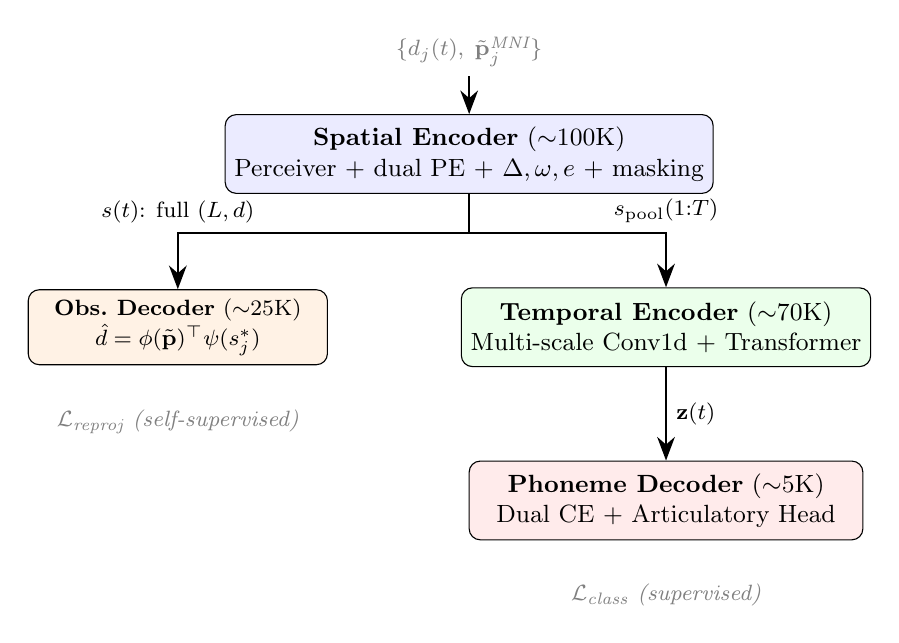
\begin{tikzpicture}[
  box/.style={draw, rounded corners, minimum width=5cm, minimum height=1cm, align=center, font=\small},
  smallbox/.style={draw, rounded corners, minimum width=3.8cm, minimum height=0.8cm, align=center, font=\footnotesize},
  arrow/.style={-{Stealth[length=3mm]}, thick},
  label/.style={font=\footnotesize\itshape, text=gray}
]

\node[box, fill=blue!8] (spatial) at (0, 0) {\textbf{Spatial Encoder} (${\sim}$100K)\\Perceiver + dual PE + $\Delta, \omega, e$ + masking};

\node[smallbox, fill=orange!10] (obs) at (-3.7, -2.2) {\textbf{Obs.\ Decoder} (${\sim}$25K)\\$\hat{d} = \phi(\tilde{\bfp})^\top\psi(s_j^*)$};

\node[box, fill=green!8] (temporal) at (2.5, -2.2) {\textbf{Temporal Encoder} (${\sim}$70K)\\Multi-scale Conv1d + Transformer};

\node[box, fill=red!8] (phoneme) at (2.5, -4.4) {\textbf{Phoneme Decoder} (${\sim}$5K)\\Dual CE + Articulatory Head};

\node[label] (input) at (0, 1.3) {$\{d_j(t),\; \tilde{\bfp}_j^{\text{MNI}}\}$};

\draw[arrow] (input) -- (spatial);
\draw[arrow] (spatial.south) -- ++(0,-0.5) -| (obs.north) node[midway, above, font=\footnotesize] {$s(t)$: full $(L,d)$};
\draw[arrow] (spatial.south) -- ++(0,-0.5) -| (temporal.north) node[midway, above, font=\footnotesize] {$s_{\text{pool}}(1{:}T)$};
\draw[arrow] (temporal) -- (phoneme) node[midway, right, font=\footnotesize] {$\bfz(t)$};

\node[label] at (-3.7, -3.4) {$\mathcal{L}_{\text{reproj}}$ (self-supervised)};
\node[label] at (2.5, -5.6) {$\mathcal{L}_{\text{class}}$ (supervised)};

\end{tikzpicture}
\end{center}

\begin{equation}
\boxed{\mathcal{L} = \mathcal{L}_{\text{class}} + \lambda \cdot \mathcal{L}_{\text{reproj}}}
\end{equation}

\textbf{Precedent for combined supervised + self-supervised losses.} This pattern is standard in settings where supervised labels are scarce and geometric structure provides additional signal:
\begin{itemize}[leftmargin=2em]
\item \textbf{NeRF / 3DGS}: photometric reconstruction loss (self-supervised: ``render what the camera should see'') + semantic labels when available. Our reprojection loss is the direct analog of photometric loss.
\item \textbf{Monocular depth estimation}: photometric consistency (self-supervised) + supervised depth loss when ground truth exists.
\item \textbf{Multi-task learning}: auxiliary reconstruction objectives alongside the primary classification loss, standard when labeled data is limited.
\end{itemize}
The reprojection loss regularizes the spatial encoder to learn geometrically coherent representations that supervised labels alone cannot enforce with only 1300 trials. The annealing $\lambda: 0.5 \to 0.1$ prioritizes geometric structure early (when the encoder needs spatial inductive bias) and classification later (when discriminative features matter most).

\begin{table}[ht!]\centering\small
\begin{tabular}{@{}lrl@{}}
\toprule
\textbf{Module} & \textbf{Params} & \textbf{Role} \\
\midrule
Spatial encoder & ${\sim}$100K & Invert observation function \\
Observation decoder & ${\sim}$25K & Forward model (reprojection) \\
Temporal encoder & ${\sim}$70K & Dynamics modeling \\
Phoneme decoder & ${\sim}$5K & Classification \\
\midrule
\textbf{Total shared} & $\mathbf{{\sim}200}$\textbf{K} & \\
Per-patient ($\times 10$) & 700 & Registration + identity \\
\textbf{Grand total} & $\mathbf{{\sim}201}$\textbf{K} & (cf.\ current pipeline: 122K) \\
\bottomrule
\end{tabular}
\end{table}


%% ====================================================================
%%  PART IV: TRAINING, EVALUATION, AND EXPERIMENTAL DESIGN
%% ====================================================================

\part{Training, Evaluation, and Experimental Design}

\section{Training Pipeline}

\subsection{Phase 1: Source patient training (supervised + reprojection)}

9 source patients, ${\sim}1315$ labeled trials. Each batch:
\begin{enumerate}[leftmargin=2em]
\item \textbf{Spatial encoding}: construct tokens, mask 20--40\% electrodes, Perceiver $\to s(t)$, attention pooling $\to s_{\text{pool}}(t)$.
\item \textbf{Reprojection}: decoder predicts all electrodes (including masked) from position-local latents $s_j^*(t)$; compute $\mathcal{L}_{\text{reproj}}$ (or $\mathcal{L}_{\text{reproj}}^{\text{UQ}}$).
\item \textbf{Temporal encoding}: $s_{\text{pool}}(1{:}T) \to$ multi-scale $\to$ transformer $\to \bfz(t)$.
\item \textbf{Classification}: dual head $\to \mathcal{L}_{\text{class}}$.
\item \textbf{Total}: $\mathcal{L} = \mathcal{L}_{\text{class}} + \lambda \mathcal{L}_{\text{reproj}}$ ($\lambda$: $0.5 \to 0.1$ annealed).
\end{enumerate}

\textbf{Optimizer}: AdamW with differential LR:
\begin{itemize}[leftmargin=2em]
\item Shared parameters: $10^{-3}$
\item Virtual positions, $\Delta$, $\omega$: $3 \times 10^{-4}$ (slow---geometric stability)
\item Patient $e$: $10^{-3}$
\end{itemize}

Linear warmup (20 epochs) $\to$ cosine decay. Weight decay $10^{-4}$. Gradient clipping 5.0. Batch size 16. Early stopping on held-out 20\% source validation, patience 7.

\subsection{Phase 2: Target adaptation (LP-FT)}

Per CV fold on target patient (5-fold grouped-by-token):
\begin{enumerate}[leftmargin=2em]
\item \textbf{Linear probe}: freeze encoder, train decoder + $\Delta^{(\text{target})} + \omega^{(\text{target})} + e^{(\text{target})}$. Initialize $e = \text{mean}(e^{(\text{source})})$. 150 epochs. Loss: $\mathcal{L}_{\text{class}} + 0.1 \cdot \mathcal{L}_{\text{reproj}}$. \textbf{Best checkpoint selected on inner validation split} (20\% of training fold held out).
\item \textbf{Fine-tune}: unfreeze encoder at $0.1\times$ LR. 100 epochs, patience 7. Best checkpoint by inner validation.
\end{enumerate}

\subsection{Phase 3 (optional): Transductive reprojection pre-training}\label{sec:phase3}

Pre-train spatial encoder + observation decoder using $\mathcal{L}_{\text{reproj}}$ only.

\textbf{Protocol distinction.} This phase uses unlabeled neural data for self-supervised pre-training. If the target patient's unlabeled data is included, this is a \textbf{transductive} protocol---the model sees target recordings before supervised evaluation. Two regimes must be reported separately:

\begin{enumerate}[leftmargin=2em]
\item \textbf{Strict LOPO}: pre-training uses only source patient data. Target patient is completely held out until Phase~2.
\item \textbf{Transductive SSL}: pre-training includes target patient's unlabeled recordings (no labels, but the model sees the distribution). This is legitimate but \textbf{not comparable to strict LOPO} without explicit disclosure.
\end{enumerate}

Phase~1 is then initialized from pre-trained weights.


\section{Evaluation Protocol}\label{sec:eval-regimes}

\subsection{Three evaluation regimes}

The cross-patient setting admits three regimes of increasing difficulty. The scientific claim differs across regimes, and results should never be compared across regimes without explicit acknowledgment:

\begin{enumerate}[leftmargin=2em]
\item \textbf{Zero-shot transfer.} Train on sources (Phase 1). Evaluate on target with no adaptation. Target-specific parameters are initialized as: $\Delta^{(\text{target})} = \mathbf{0}$, $\omega^{(\text{target})} = \mathbf{0}$, $e^{(\text{target})} = \frac{1}{K}\sum_{k=1}^{K} e^{(k)}$ (mean source embedding). These values are frozen---no gradient updates from target data. Claim: ``the shared model generalizes to unseen electrode configurations using only MNI coordinates.'' This is the strongest scientific claim but likely yields poor PER at our data scale, since the mean source embedding is a crude proxy for patient-specific physiology.

\item \textbf{LP-FT adaptation} (primary evaluation). Phase 1 $\to$ Phase 2 (linear probe + fine-tune on target folds). Claim: ``source training provides a useful initialization for few-shot target adaptation.'' This is our primary regime---it matches the clinical scenario where a short calibration session is available.

\item \textbf{Transductive SSL + LP-FT.} Phase 3 (with target unlabeled data) $\to$ Phase 1 $\to$ Phase 2. Claim: ``unlabeled target data further improves adaptation.'' Reported separately from regime 2.
\end{enumerate}

\subsection{Metrics and protocol}

PER via edit distance, grouped-by-token 5-fold CV. Full recipe: weighted $k$-NN ($k{=}10$, cosine), TTA 16, dual head, source $k$-NN at $0.5\times$ weight. Conformal prediction sets as interpretability output.

\textbf{Checkpoint selection.} Within each CV fold, the best checkpoint is selected on a \textbf{held-out inner validation split} (20\% of the training portion of that fold). The test portion of the fold is never used for model selection. This is standard nested cross-validation, not test-set leakage.


\section{Ablation Experiments}

\begin{table}[ht!]\centering\small
\begin{tabular}{@{}clp{7.0cm}@{}}
\toprule
\textbf{ID} & \textbf{Ablation} & \textbf{Question} \\
\midrule
A1 & MNI PE present/absent & \textbf{Central}: do MNI coordinates help? \\
 & \quad a. Current Conv2d + BiGRU baseline & $\to$ 0.762 (LP-FT regime) \\
 & \quad b. Perceiver, random-init positions & $\to$ architecture benefit \\
 & \quad c. Perceiver + MNI PE & $\to$ MNI benefit \\
 & \quad d. (c) + reprojection loss & $\to$ reprojection benefit \\
\midrule
A2 & \textbf{Population-level (all patients)} & \textbf{Is the 0.76 wall S14-specific?} \\
\midrule
A3 & Per-patient params & $\Delta$ only / $+\omega$ / $+e$ / position-dep.\ $e$ \\
A4 & Virtual electrode count & $L \in \{4, 8, 16, 32\}$ \\
A5 & Reprojection weight & $\lambda \in \{0, 0.01, 0.1, 0.5\}$ \\
A6 & Cross-task pooling & $+$ Duraivel data (architecture-independent) \\
A7 & Reprojection loss & Beta-NLL vs.\ MSE-only \\
A8 & Spatial readout & MaxPool / attention pool / full $(L,d)$ \\
A9 & Bilinear vs.\ MLP decoder & $\phi^\top\psi$ vs.\ $\text{MLP}([\tilde{\bfp}; e; s_j^*])$ \\
A10 & Temporal backbone & Transformer vs.\ BiGRU (+ stride re-valid.) \\
\bottomrule
\end{tabular}
\end{table}


\section{Experimental Priorities}\label{sec:priorities}

The document's own evidence suggests a clear priority ordering that should be stated transparently:

\begin{enumerate}[leftmargin=2em]
\item \textbf{Cross-task data pooling} (A6). Lowest risk, highest confidence. Same phonemes, overlapping patients, validated by Duraivel 2025~\cite{duraivel2025}. Directly addresses target-data scarcity. Can be tested with the current pipeline \textbf{and} the new architecture. Should be pursued first, in parallel with coordinate sourcing.

\item \textbf{Population-level evaluation} (A2). Pure methodology fix. Required to determine whether the 0.76 wall is S14-specific (55-experiment overfitting) or universal. Must be the \textbf{primary success criterion}, not just an ablation. Zero architectural risk.

\item \textbf{MNI coordinate-based architecture} (A1, this document). A working hypothesis. The evidence that spatial alignment is THE binding constraint is suggestive but unvalidated: it has not been isolated from data scarcity, measurement noise, or S14-specific effects (Section~\ref{sec:wall}). The architectural investment is justified by: (a)~MNI coordinates are currently unused information; (b)~the observation function formulation provides a principled framework; (c)~every component has a structural precedent in related domains (vision, neural BCI). But the hypothesis could be wrong---coordinates may not help if the wall is data-limited rather than alignment-limited.
\end{enumerate}

\textbf{The architecture is the most speculative of the three paths}---highest risk but also highest novelty. The document should not obscure this priority ordering.


\section{Success Criteria}\label{sec:success}

\textbf{Primary criterion (population-level):}
\begin{itemize}[leftmargin=2em]
\item Mean PER across all patients improves over current LOPO baseline, evaluated across ${\geq}3$ seeds, in the LP-FT regime.
\item The MNI coordinate hypothesis is tested by \textbf{specific paired comparisons} within the A1 ablation family: \textbf{A1c vs.\ A1b} isolates MNI benefit (controlling for Perceiver architecture), and \textbf{A1d vs.\ A1c} isolates reprojection benefit (controlling for MNI). Only these paired comparisons provide evidence for or against the coordinate hypothesis---the overall A1c/d vs.\ A1a comparison confounds architecture and coordinates.
\end{itemize}

\textbf{S14 pilot evidence (exploratory only):}
\begin{itemize}[leftmargin=2em]
\item S14 results serve as \textbf{pilot directional evidence} during development. They are contaminated by 55+ prior experiments and should not be used as definitive success criteria.
\item If population-level results disagree with S14 pilot results, the population-level results take precedence.
\end{itemize}

\textbf{Interpretability (qualitative validation):}
\begin{itemize}[leftmargin=2em]
\item Virtual electrode positions cluster over known speech motor regions.
\item Learned $\Delta^{(i)}, \omega^{(i)}$ are weak proxies for registration error unless independently validated (e.g., against known registration quality metrics). They may also absorb physiology, coverage differences, or optimization artifacts. Correlation with tumor status would be suggestive but not conclusive.
\item Spatial tuning vectors $\phi(\bfp)$ recover articulatory somatotopy when visualized.
\item Electrode masking patterns: which electrodes, when dropped, cause the largest reconstruction error---reveals which positions carry the most unique information.
\end{itemize}


\section{Available Data}

\subsection{Cohort accounting}

One table to resolve all patient references in this document:

\begin{table}[ht!]\centering\small
\begin{tabular}{@{}lllccc@{}}
\toprule
\textbf{Cohort} & \textbf{Patients} & \textbf{Trials} & \textbf{Tumor} & \textbf{MNI} & \textbf{Usage} \\
\midrule
\multicolumn{6}{@{}l}{\textit{PS task (primary): 12 usable patients (S18 excluded --- no preprocessed data)}} \\
\quad Source (Spalding 8) & S22,S23,S26,S33, & ${\sim}$1162 & 4/9 & \textdagger & Source train \\
 & S39,S58,S62 + 2 non-Spalding & & & & \\
\quad S14 (target, pilot) & S14 & 153 & No & \textdagger & Target eval \\
\quad Additional PS & S16,S32,S36,S57 & ${\sim}$400 & 2/4 & \textdagger & Future source \\
\midrule
\multicolumn{6}{@{}l}{\textit{Pseudo-word repetition (Duraivel 2025): 3 intra-op $\mu$ECoG overlap}} \\
\quad Cross-task & 3 pts (= S58,S26,S14/S22) & 156--208 ea. & Mixed & \textdagger & More data \\
\midrule
\multicolumn{6}{@{}l}{\textit{Lexical task: 13 usable patients, different task (28 phonemes)}} \\
\quad Lexical patients & S41,S45,...,S76 & Varies & Mixed & \textdagger & Future source \\
\midrule
\textbf{Total unique} & ${\sim}$\textbf{25 patients} & & 6/12 PS & & \\
\bottomrule
\end{tabular}
\end{table}

\noindent \textdagger\ MNI coordinates: expected to be extractable from BioImage Suite (DBS patients) or Brainlab (tumor patients) electrode reconstruction outputs stored in ECoG\_Recon on Box. \textbf{Not yet extracted for this project}---status must be confirmed with Greg Cogan. Fallback: scaled ACPC grid positions (retains within-patient structure, loses cross-patient alignment).

\textbf{Note}: S32 and S36 are the same patient recorded twice (confirmed from data inspection). The 12 ``usable PS patients'' count reflects 11 unique individuals + 1 duplicate.

\subsection{Data sources}

\begin{table}[ht!]\centering\small
\begin{tabular}{@{}llc@{}}
\toprule
\textbf{Data source} & \textbf{Usage} & \textbf{Risk} \\
\midrule
PS task HGA (9 source pts) & Phase 1 source training & -- \\
S14 HGA (153 trials) & Phase 2 target eval (pilot) & -- \\
Cross-task (3 pts, 156--208 trials) & \textbf{Priority 1: more data} & Low \\
MNI coordinates (all pts) & Perceiver architecture & Medium \\
Continuous recordings (${\sim}168$\,min) & Phase 3 reproj.\ SSL & Medium \\
Lexical task (13 pts) & Additional source pool & Medium \\
\bottomrule
\end{tabular}
\end{table}


\section{Risk Assessment}

\begin{table}[ht!]\centering\small
\begin{tabular}{@{}p{0.33\textwidth}cp{0.44\textwidth}@{}}
\toprule
\textbf{Risk} & \textbf{Sev.} & \textbf{Mitigation} \\
\midrule
MNI coordinates unavailable & High & Fallback to random-init positions \\
MNI alignment too imprecise & High & Ablation A1; learnable $\alpha$ adapts blur \\
Reprojection competes with classification & Medium & $\lambda$ ablation A5; $\lambda{=}0$ fallback \\
Perceiver overfits (200K, 1300 trials) & Medium & Masking; early stopping; reprojection reg. \\
Bilinear separability too restrictive & Medium & Ablation A9: MLP fallback \\
Per-patient params insufficient for tumor & Medium & Ablation A3; position-dep.\ $e$ option \\
Virtual electrodes collapse & Low & Initialize across convex hull; monitor \\
\bottomrule
\end{tabular}
\end{table}


\section{Summary}

This document formalizes cross-patient speech decoding as \textbf{multi-view neural field reconstruction}, a structural analogy to 3D vision that is generative but not a substitute for empirical validation (Section~\ref{sec:disanalogies}).

The implemented model (Eq.~\ref{eq:implemented}) is patient-conditioned: it conditions on patient identity $e^{(i)}$ and learned geometric corrections $\Delta^{(i)}, \omega^{(i)}$, relaxing the idealized shared observation function. The architecture produces two distinct representations: $s(t)$ (per-frame spatial summary, trained via reprojection) and $\bfz(t)$ (temporally-refined state, trained via classification). The observation decoder uses position-weighted aggregation of virtual electrode outputs (Eq.~\ref{eq:local-agg}), preserving the spatial decomposition that motivates virtual electrodes. It employs a bilinear factorization that assumes separability between spatial tuning and articulatory activation---a structural hypothesis requiring empirical validation (ablation A9).

Total budget: ${\sim}200$K shared + 70 per patient. The architecture is the most speculative of three research paths (Section~\ref{sec:priorities}); its value lies in principled exploitation of currently unused coordinate information, with every structural assumption marked for empirical test.


% ── Bibliography ──────────────────────────────────────────
\begin{thebibliography}{99}\raggedright

\bibitem{singh2025}
Singh, A., Thomas, T., Li, J., Hickok, G., Pitkow, X., \& Tandon, N.\ (2025).
Transfer learning via distributed brain recordings enables reliable speech decoding.
\textit{Nature Communications}, 16, 8749.
\texttt{doi:10.1038/s41467-025-63825-0}

\bibitem{willett2023}
Willett, F.R., et al.\ (2023).
A high-performance speech neuroprosthesis.
\textit{Nature}, 620, 1031--1036.

\bibitem{metzger2023}
Metzger, S.L., et al.\ (2023).
A high-performance neuroprosthesis for speech decoding and avatar control.
\textit{Nature}, 620, 1037--1046.

\bibitem{wu2025}
Wu, R., Berezutskaya, J., Freudenburg, Z.V., \& Ramsey, N.F.\ (2025).
Across-speaker articulatory reconstruction from sensorimotor cortex for generalizable brain-computer interfaces.
\textit{bioRxiv}.
\texttt{doi:10.1101/2025.10.08.680888}

\bibitem{chen2025}
Chen, J., Chen, X., Wang, R., Le, C., Khalilian-Gourtani, A., Yu, L., Dugan, P., Friedman, D., Doyle, W., Devinsky, O., Wang, Y., \& Flinker, A.\ (2025).
Transformer-based neural speech decoding from surface and depth electrode signals.
\textit{Journal of Neural Engineering}, 22(1), 016017.
\texttt{doi:10.1088/1741-2552/ada741}

\bibitem{safaie2023}
Safaie, M., et al.\ (2023).
Preserved neural dynamics across animals performing similar behaviour.
\textit{Nature Neuroscience}, 26, 714--724.

\bibitem{gallego2020}
Gallego, J.A., et al.\ (2020).
Long-term stability of cortical population dynamics underlying consistent behavior.
\textit{Nature Neuroscience}, 23, 260--270.

\bibitem{bouchard2013}
Bouchard, K.E., et al.\ (2013).
Functional organization of human sensorimotor cortex for speech articulation.
\textit{Nature}, 495, 327--332.

\bibitem{anumanchipalli2019}
Anumanchipalli, G.K., et al.\ (2019).
Speech synthesis from neural decoding of spoken sentences.
\textit{Nature}, 568, 493--498.

\bibitem{spalding2025}
Spalding, Z., Duraivel, S., Rahimpour, S., Wang, C., Barth, K., Schmitz, C., Lad, S.P., Friedman, A.H., Southwell, D.G., Viventi, J., \& Cogan, G.B.\ (2025).
Shared latent representations of speech production for cross-patient speech decoding.
\textit{bioRxiv}.
\texttt{doi:10.1101/2025.08.21.671516}

\bibitem{duraivel2023}
Duraivel, S., Rahimpour, S., Chiang, C.-H., et al.\ (2023).
High-resolution neural recordings improve the accuracy of speech decoding.
\textit{Nature Communications}, 14, 6938.
\texttt{doi:10.1038/s41467-023-42555-1}

\bibitem{duraivel2025}
Duraivel, S., Rahimpour, S., Barth, K., et al.\ (2025).
Distinct neural processes link speech planning and execution.
\textit{bioRxiv}.
\texttt{doi:10.1101/2024.10.07.617122}

\bibitem{seitzer2022}
Seitzer, M., et al.\ (2022).
On the pitfalls of heteroscedastic uncertainty estimation with probabilistic neural networks.
\textit{ICLR 2022}.

\bibitem{gal2016}
Gal, Y.\ \& Ghahramani, Z.\ (2016).
Dropout as a Bayesian approximation: Representing model uncertainty in deep learning.
\textit{ICML 2016}.

\bibitem{angelopoulos2021}
Angelopoulos, A.N.\ \& Bates, S.\ (2021).
A gentle introduction to conformal prediction and distribution-free uncertainty quantification.
\textit{arXiv:2107.07511}.

\bibitem{wang2025}
Wang, J., Chen, M., Karaev, N., Vedaldi, A., Rupprecht, C., \& Novotny, D.\ (2025).
VGGT: Visual Geometry Grounded Transformer.
\textit{CVPR 2025}.
\texttt{arXiv:2503.11651}

\bibitem{jin2024}
Jin, H., et al.\ (2024).
LVSM: A large view synthesis model with minimal scene representations.
\textit{ICLR 2025}.

\bibitem{xiong2024}
Xiong, Z., et al.\ (2024).
MMGN: Multi-scale multi-modal graph network for spatiotemporal field reconstruction.
\textit{ICLR 2024}.

\bibitem{truong2023}
Truong, P., et al.\ (2023).
SPARF: Neural radiance fields from sparse and noisy poses.
\textit{CVPR 2023}.

\bibitem{jha2023}
Jha, A.H., et al.\ (2023).
Senseiver: Perceiver IO for sparse sensor field reconstruction.
\textit{Nature Machine Intelligence}.

\bibitem{jaegle2021}
Jaegle, A., et al.\ (2021).
Perceiver: General perception with iterative attention.
\textit{ICML 2021}.

\bibitem{rvm2025}
Tong, Z., et al.\ (2025).
Recurrent Video Masked Autoencoders.
\textit{arXiv:2512.13684}.

\bibitem{maest2025}
Li, X., et al.\ (2025).
3D masked autoencoder with spatiotemporal transformer for modeling of 4D fMRI data.
\textit{Medical Image Analysis}, 103633.
\texttt{doi:10.1016/j.media.2025.103633}

\bibitem{videomamba2025}
Li, K., et al.\ (2025).
Video Mamba Suite: State space model as a versatile alternative for video understanding.
\textit{International Journal of Computer Vision}.
\texttt{doi:10.1007/s11263-025-02597-y}

\bibitem{videomae2022}
Tong, Z., et al.\ (2022).
VideoMAE: Masked autoencoders are data-efficient learners for self-supervised video pre-training.
\textit{NeurIPS 2022 Spotlight}.

\bibitem{qi2017}
Qi, C.R., Su, H., Mo, K., \& Guibas, L.J.\ (2017).
PointNet: Deep learning on point sets for 3D classification and segmentation.
\textit{CVPR 2017}.

\bibitem{zhao2021}
Zhao, H., Jiang, L., Jia, J., Torr, P., \& Koltun, V.\ (2021).
Point Transformer.
\textit{ICCV 2021}.

\end{thebibliography}

\end{document}
